\bookpart{集合函数与子集选择}{Set Functions and Subset Selection}
\label{part:set-functions-subset-selection}

\BookPartGuide{%
前一部分选择的是路径、生成树、流和匹配，候选对象都带有特定的图结构。许多选择问题只要求从有限个候选中挑出一组：安装哪些传感器、保留哪些特征、把哪些顶点分到一侧。这时被评价的是整组选择，而组内元素的重叠、替代或配合会改变总分。本部分把候选放进一个有限的底集，研究怎样评价它的子集，以及怎样利用评价的结构完成选择；底集可以是图的顶点或边，也可以与图无关。

第一章建立共同语言。集合函数给每个子集一个值，边际增益记录加入一个元素前后的变化；单调性、模性和次模性分别用边际增益回答三个不同的问题：新增元素会不会降低评价，各元素的贡献是否固定，收益是否随已选集合增大而递减。同一章还处理一个与选择无关的问题：已知每个子集的累计值，怎样由Möbius反演恢复各子集自身的贡献。这个问题只用有限求和与包含关系，不需要单调或次模假设。

后两章分别处理两类选择。第二章在“至多选$k$个”或“总成本不超过预算”的约束下最大化目标，研究逐轮加入元素的贪心规则；目标归一化、单调且次模时，基数约束下的贪心有固定比例的近似保证，预算约束下的简单比值规则却没有。第三章转向最小化：目标由一元项和成对项组成、每个成对项满足次模条件时，全部配置的成本可以写成割容量，再用第~\ref{chap:max-flow-min-cut}章的最大流最小割精确求解。

阅读时要分清三组东西。第一，函数性质各管一件事，次模不蕴含单调，单调也不蕴含次模。第二，贪心规则本身、它的惰性实现和它的近似保证是三件事：规则在任何集合函数上都能执行，惰性实现与普通贪心选出同样元素要靠次模性，比例保证还要加上归一化、单调和基数约束。第三，最大化得到的是有保证的近似解，成对二值最小化在条件满足时得到精确解；条件不满足或附加了其他约束时，两种方法都不能直接沿用。}

\chapter{集合函数与子集累计}
\label{chap:set-functions}
\label{chap:graph-set-functions}

在一片区域里安装传感器时，每个候选位置覆盖一块范围，相邻位置的覆盖范围往往重叠。选定一组位置后，有意义的是这组位置合起来覆盖了多少，而不是各自覆盖面积的简单相加。从一批特征里挑出一组、从一张图里挑出一部分顶点，评价的也都是整组选择。本章要回答两个问题：怎样描述这种对整组的评价，以及评价具有哪些结构可以供后面的选择算法利用；另外，已知每个子集的累计评价时，怎样恢复各个子集自身的贡献。

前两节建立描述子集评价的语言。第~\ref{sec:graph-set-function-basics}节把“给子集赋值”写成集合函数，用指示向量换一种方式索引子集，并用加入一个元素前后的评价差定义边际增益。第~\ref{sec:graph-set-function-properties}节用边际增益区分单调性、模性和次模性，并说明它们互不蕴含。

第~\ref{sec:comb-cumulative-inversion}节处理另一项任务：由累计值恢复自身贡献。它只用有限求和与包含关系，不依赖前一节的任何性质，也不是后两章选择算法的前提。本章用到卷一的幂集计数、裂项求和、偏序关系、有限和的交换次序与组合数的交错和，用到时在当地说明所需的结论。

% 第8章第1节：集合函数（集合函数的定义；子集与二值向量；边际增益）。

\section{集合函数}
\label{sec:graph-set-function-basics}

给每个元素赋一个数，只需要一张长度为元素个数的表。对整组选择打分就不同了：元素之间的重叠、替代或配合都会改变总分，分数只能直接对子集给出。所以本节以子集为自变量的函数为基本对象。选择又往往是一次加入一个元素，所以还要看加入一个元素前后分数怎样变化。

\subsection{集合函数的定义}
\label{sec:graph-setfn-definition}

图~\ref{fig:graph-setfn-sensor-coverage}是一块由上下两行、左右八列组成的区域，共$16$个格子。有四个候选传感器：$a$覆盖第$2$至$6$列的$10$个格子，$b$覆盖第$1$至$4$列的$8$个格子，$c$覆盖第$5$至$8$列的$8$个格子，$d$只覆盖左上角的$1$个格子。

选定一组传感器后，我们关心它们合起来覆盖了多少个不同的格子。记传感器$v$覆盖的格子集合为$C_v$，选定的传感器集合为$S$，覆盖量就是
\[
  F(S)=\Bigl|\bigcup_{v\in S}C_v\Bigr|.
\]
单独看，$F(\{a\})=10$，$F(\{b\})=8$。两者一起时，第$2$至$4$列被重复覆盖，所以
\[
  F(\{a,b\})=12<F(\{a\})+F(\{b\})=18.
\]
整组的价值不能由各成员的价值相加得到，因此评价必须直接以“哪些传感器被选中”为输入。本章和下一章都用这个实例做算例。

\begin{figure}[!htb]
  \centering
  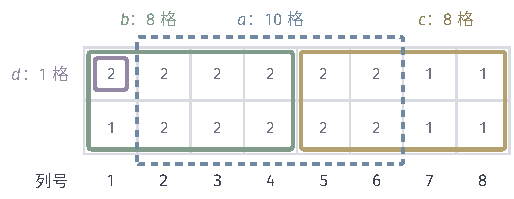
\includegraphics[width=87.027mm]{figures/01-basic-mathematics/04-graphs/tikz/c4-sensor-coverage/figure.pdf}
  \caption{贯穿本章和下一章的传感器覆盖实例。区域由$2\times 8$个格子组成；绿色框为$b$（第$1$至$4$列），黄色框为$c$（第$5$至$8$列），蓝色虚线框为$a$（第$2$至$6$列），紫色小框为$d$（左上角一格）。格内数字是覆盖该格的传感器个数，数字$2$所在的格子都被重复覆盖，因而各传感器覆盖格数之和大于它们合起来覆盖的格数。}
  \label{fig:graph-setfn-sensor-coverage}
\end{figure}

覆盖量的输入是一个子集，输出是一个实数。把这种对应一般化，就得到下面的定义。

\begin{definition}[集合函数]
\label{def:graph-setfn-set-function}
设$V$是有限集合，称为\term{底集}（ground set）。把$V$的每个子集对应到一个实数的映射
\[
  F:\mathcal P(V)\to\mathbb R
\]
称为$V$上的\term{集合函数}（set function），其中$\mathcal P(V)$是$V$的幂集。
\end{definition}

定义要求$F$在每个子集上都有值，包括空集。空集表示“什么都不选”，它的值是比较其他选择的起点：覆盖量取$F(\varnothing)=0$，一个带固定开销的评价则可能取非零值。底集中的元素可以是传感器、特征、顶点或边；集合函数本身并不要求底集带有图结构。

\paragraph{总成本与割权}
同一个子集可以按不同目的评价。给四个传感器依次指定安装成本$4,3,4,1$（对应$a,b,c,d$），总成本
\[
  c(S)=\sum_{v\in S}c_v
\]
是一个集合函数，例如$c(\{a,b\})=7$；覆盖量$F$是另一个，$F(\{a,b\})=12$。

第三个例子来自图。设$\mathcal G=(V,E)$是无向图，每条边$\{i,j\}$带非负权$w_{i,j}$。顶点子集$S$把顶点分成$S$与$V\setminus S$两侧，这就是第~\ref{sec:graph-opt-cut-property}节所说的割；那里要求两侧都非空，这里允许$S=\varnothing$或$S=V$，这时没有边跨越两侧。两端分居两侧的边的权之和
\[
  \operatorname{cut}(S)=\sum_{\{i,j\}\in E:\ |\{i,j\}\cap S|=1}w_{i,j}
\]
称为$S$的割权，它以顶点子集为自变量。

三个函数分别累计单项成本、合并覆盖范围、统计跨越两侧的边，元素之间的相互影响各不相同。下一节据此区分它们的性质。

\paragraph{取值表与求值规则}
$n$元底集的每个元素有选与不选两种可能，按乘法规则共有$2^n$个子集，所以一个集合函数的完整取值表有$2^n$项（幂集计数可参考\BookChapterRef{chap:counting}{卷一“计数”章}）。传感器实例只有$16$项。除上面的单元素值外，二元子集的覆盖量为
\[
  \begin{gathered}
  F(\{a,b\})=12,\quad F(\{a,c\})=14,\quad F(\{a,d\})=11,\\
  F(\{b,c\})=16,\quad F(\{b,d\})=8,\quad F(\{c,d\})=9,
  \end{gathered}
\]
三元子集中$\{a,b,c\}$与$\{b,c,d\}$覆盖全部$16$格；后面各节的枚举基准都从这些值读出。

底集有$50$个元素时，取值表已超过$10^{15}$项，无法存储。因此实际问题中的集合函数通常由一条规则给出：给定$S$，按规则算出$F(S)$，这样的一次计算称为一次\emph{求值}。覆盖量的规则是维护一个格子标记数组，初始全为未覆盖，依次标记$S$中各传感器覆盖的格子，最后计数。求$F(\{a,b,c\})$时，读入$b$标记第$1$至$4$列，读入$a$新增第$5$、$6$列，读入$c$新增第$7$、$8$列，共$16$格，工作量与$\sum_{v\in S}|C_v|$成正比。割权的规则是扫描全部边，工作量与边数成正比。

两种给出方式的代价不同。查表读值便宜，但表随$n$指数增长；规则不必存表，却每次读值都要计算。所以后面分析算法时，我们把求值次数和每次求值的代价分开计算，不把求值视为免费。

\subsection{子集与二值向量}
\label{sec:graph-setfn-binary-vectors}

给底集的元素固定编号$V=\{1,\ldots,n\}$。前面计算子集个数时用到，子集$S$与长度为$n$的零一记录一一对应。把这条记录写成向量$\bm x=(x_1,\ldots,x_n)\in\{0,1\}^n$，其中
\[
  x_i=\mathbb I\{i\in S\},
\]
称$\bm x$为$S$的\term{指示向量}（indicator vector）。这里$\mathbb I\{\cdot\}$是指示函数，条件成立时取$1$，否则取$0$。反过来，收集取值为$1$的坐标就恢复出子集：$S=\{i:x_i=1\}$。

集合运算在指示向量上逐坐标进行。设$S,T$的指示向量为$\bm x,\bm y$，则$|S|=\sum_ix_i$；并集、交集与补集的第$i$个坐标依次是
\[
  \max\{x_i,y_i\},\qquad \min\{x_i,y_i\}=x_iy_i,\qquad 1-x_i;
\]
包含关系$S\subseteq T$对应逐坐标的$x_i\leq y_i$。每种运算都只需扫描一遍$n$个坐标。

于是集合函数也可以写成二值向量的函数：令$f(\bm x)=F(\{i:x_i=1\})$，$f$与$F$只是同一组数值的两种索引方式。图~\ref{fig:graph-setfn-subset-binary-cube}以三元底集为例画出这一对应：八个子集恰好是立方体的八个顶点，立方体的每条边连接只差一个元素的两个子集，也就是只差一个坐标的两个向量。

\begin{figure}[!htb]
  \centering
  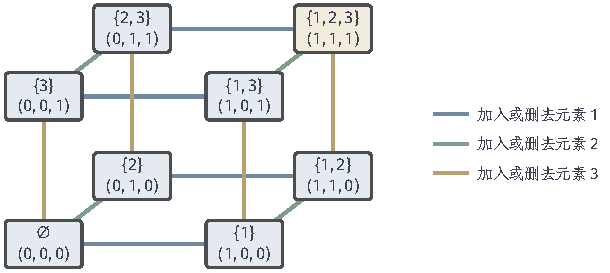
\includegraphics[width=103.209mm]{figures/01-basic-mathematics/04-graphs/tikz/c4-subset-binary-cube/figure.pdf}
  \caption{三元底集$V=\{1,2,3\}$的八个子集与指示向量$(x_1,x_2,x_3)$排成立方体的顶点。每个框上行是子集，下行是对应的向量；边的颜色表示沿这条边加入或删去哪个元素，也就是改变哪个坐标。沿任一条边向上走一步，就是在当前子集中加入一个元素。}
  \label{fig:graph-setfn-subset-binary-cube}
\end{figure}

这一改写只换了表示方式，并没有带来额外结构。写成$f(\bm x)$之后，$f$不一定是各坐标的函数之和，也不一定能分解成只读取少数坐标的局部项；在$\{0,1\}^n$上谈连续性或求导也没有意义。第~\ref{chap:pairwise-binary-minimization}章和第~\ref{part:graph-dynamic-programming}部分讨论的，正是函数确实具有某种局部分解时可以怎样利用它。

\subsection{边际增益}
\label{sec:graph-setfn-marginal-gain}

选择子集时，最直接的问题是：在已经选好的集合上再加一个元素，评价会改变多少。

\begin{definition}[边际增益]
\label{def:graph-setfn-marginal-gain}
设$F$是$V$上的集合函数，$S\subseteq V$，$v\in V\setminus S$。称
\begin{equation}
  \Delta(v\mid S)=F(S\cup\{v\})-F(S)
  \label{eq:graph-setfn-marginal-gain}
\end{equation}
为元素$v$相对于集合$S$的\term{边际增益}（marginal gain）。
\end{definition}

边际增益同时依赖新元素和已选集合。图~\ref{fig:graph-setfn-marginal-gain-overlap}比较同一个传感器$c$在两种情况下的增益。从空集加入时，$c$的$8$个格子都是新覆盖的；已经选了$a$之后，$c$的第$5$、$6$列已被$a$覆盖，只有第$7$、$8$列的$4$个格子是新的。两个增益分别是
\[
  \Delta(c\mid\varnothing)=8,\qquad \Delta(c\mid\{a\})=4.
\]
所以谈论一个元素“值多少”时，必须说明是相对于哪个已选集合。

\begin{figure}[!htb]
  \centering
  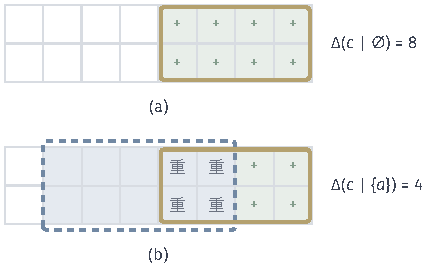
\includegraphics[width=81.217mm]{figures/01-basic-mathematics/04-graphs/tikz/c4-marginal-gain-overlap/figure.pdf}
  \caption{同一传感器$c$（黄色框）的边际增益随已选集合变化。(a) 已选集合为空，$c$覆盖的$8$个格子（绿色，标“$+$”）全部是新覆盖；(b) 已选$\{a\}$（蓝色底与蓝色虚线框），$c$与$a$重叠的第$5$、$6$列（标“重”）不再计数，只有第$7$、$8$列的$4$个格子是新覆盖。}
  \label{fig:graph-setfn-marginal-gain-overlap}
\end{figure}

\paragraph{逐个加入的累计}
边际增益只描述一步。两个有包含关系的集合相差若干元素时，把多出的元素逐个加入，函数的总变化就是一串边际增益之和。设$A\subseteq B\subseteq V$，把$B\setminus A$中的元素按任意次序排成$v_1,\ldots,v_r$，记$A_0=A$，$A_k=A\cup\{v_1,\ldots,v_k\}$。于是$A_r=B$，并且
\begin{equation}
  \begin{aligned}
  F(B)-F(A)&=\sum_{k=1}^{r}\bigl(F(A_k)-F(A_{k-1})\bigr)\\
  &=\sum_{k=1}^{r}\Delta(v_k\mid A_{k-1}).
  \end{aligned}
  \label{eq:graph-setfn-telescoping}
\end{equation}
第一个等号是裂项求和：中间的$F(A_1),\ldots,F(A_{r-1})$各出现一次正号、一次负号而抵消，只剩$F(A_r)-F(A_0)$（有限和的裂项可参考\BookChapterRef{chap:sets-relations-maps}{卷一“集合、关系与映射”章}）。第二个等号成立，是因为$A_k=A_{k-1}\cup\{v_k\}$且$v_k\notin A_{k-1}$，每一项正是一个有定义的边际增益。下一节判别性质、第~\ref{sec:graph-cardinality-selection}节分析贪心算法，用的都是这个式子。

在传感器实例中取$A=\varnothing$、$B=\{a,b,c\}$。按$a,c,b$的次序加入：$a$覆盖$10$格，$c$补上第$7$、$8$列的$4$格，$b$只补上第$1$列的$2$格，增益依次是$10,4,2$。按$b,c,a$的次序加入：$b$覆盖$8$格，$c$与$b$不重叠，补上$8$格，此时$16$格已全部覆盖，$a$的增益为$0$，增益依次是$8,8,0$。两种次序的增益之和都等于同一个值：
\[
  10+4+2=8+8+0=16=F(\{a,b,c\}).
\]
总变化由两端的集合决定，单步增益则取决于走哪条路线。

单步增益的大小也不能说明一个元素是否值得选。在空集上，$a$的增益$10$是四个传感器中最大的，但只能选两个传感器时，最好的组合是覆盖全部$16$格的$\{b,c\}$，并不包含$a$。第~\ref{sec:graph-cardinality-selection}节会具体比较这两者。

% 第8章第2节：集合函数的性质（单调性；模性；次模性；性质之间的关系）。

\section{集合函数的性质}
\label{sec:graph-set-function-properties}

上一节的三个函数在加入一个元素时表现不同：加入传感器不会减少覆盖，但新增的覆盖可能越来越少；加入一项成本总是增加固定的数额；把一个顶点移到$S$一侧，割权可能增加也可能减少。这三种表现分别对应单调性、模性和次模性。

三者都可以用边际增益判别，但各自回答一个不同的问题：新增元素会不会降低评价，每个元素的贡献是否固定，收益是否随已选集合增大而递减。所以一个函数可以具备其中任意几项而缺少其他几项，本节最后用反例和对照表核对这一点。

\subsection{单调性}
\label{sec:graph-setfn-monotonicity}

多装一个传感器，覆盖的格子只会增加或保持不变。把这一性质写成子集之间的比较，就是下面的定义。

\begin{definition}[单调非减]
\label{def:graph-setfn-monotone}
若对任意$A\subseteq B\subseteq V$都有$F(A)\leq F(B)$，称集合函数$F$\term{单调非减}（monotone nondecreasing），简称单调。
\end{definition}

定义比较的是任意两个有包含关系的子集，直接检查要考虑很多对。借助式~\eqref{eq:graph-setfn-telescoping}，可以化成只检查单个元素的条件：$F$单调，当且仅当对每个$S\subseteq V$和每个$v\notin S$都有
\[
  \Delta(v\mid S)\geq0.
\]

必要性只需取$A=S$、$B=S\cup\{v\}$。充分性：对任意$A\subseteq B$，式~\eqref{eq:graph-setfn-telescoping}把$F(B)-F(A)$写成若干个边际增益之和，每一项都非负，所以$F(A)\leq F(B)$。

覆盖量是单调的，因为加入$v$后新增的格子数
\[
  \Delta(v\mid S)=\Bigl|C_v\setminus\bigcup_{u\in S}C_u\Bigr|
\]
不会是负数。

但目标中含有覆盖量，并不保证整个目标单调。把覆盖量减去安装成本，得到净收益$G(S)=F(S)-c(S)$。比较两个集合：
\[
  G(\{b\})=8-3=5,\qquad G(\{b,d\})=8-4=4.
\]
$d$覆盖的那一格已被$b$覆盖，加入$d$不增加覆盖，却多花$1$个单位成本，所以净收益下降。

\paragraph{非负性与归一化}
函数值全为非负，也不能推出单调。在二元底集$\{1,2\}$上取
\[
  F(\varnothing)=1,\quad F(\{1\})=3,\quad F(\{2\})=2,\quad F(\{1,2\})=2,
\]
四个值都是正数，但$\Delta(2\mid\{1\})=2-3=-1<0$，所以它不单调。

反过来，单调也不能推出$F(\varnothing)=0$：常数函数$F\equiv5$是单调的。$F(\varnothing)=0$称为\emph{归一化}，它是一项约定，不是函数的固有性质：对任意集合函数，减去常数$F(\varnothing)$就得到归一化的函数，而所有边际增益保持不变。归一化且单调的函数必然处处非负，因为$F(S)\geq F(\varnothing)=0$。

\subsection{模性}
\label{sec:graph-setfn-modularity}

总成本$c(S)$具有最简单的结构：每个元素贡献一个固定的数，彼此互不影响。一般地，取常数$c_0$和每个元素的权$w_v$，令
\begin{equation}
  F(S)=c_0+\sum_{v\in S}w_v .
  \label{eq:graph-setfn-modular-form}
\end{equation}
这时对任意$S$和$v\notin S$都有
\[
  \Delta(v\mid S)=w_v,
\]
增益与已选集合无关。由上一小节的判别条件，这样的$F$单调当且仅当每个$w_v\geq0$；常数$c_0$不影响任何边际增益。

给定一个集合函数，要判断它是否具有这种固定贡献的形式，可以逐个检查边际增益是否与$S$无关；更紧凑的办法是检查一个只涉及四个函数值的等式。

对形如式~\eqref{eq:graph-setfn-modular-form}的函数和任意两个子集$A,B$，比较$F(A)+F(B)$与$F(A\cup B)+F(A\cap B)$。两边都含两个常数$c_0$，只需逐个元素比较权重被计了几次。对一个元素$v$：若$v$同时属于$A$和$B$，则$w_v$在左边计两次，在右边的并集与交集中也各计一次；若$v$只属于其中一个，则$w_v$在两边都只计一次；若$v$都不属于，则两边都不计。所以
\begin{equation}
  F(A)+F(B)=F(A\cup B)+F(A\cap B).
  \label{eq:graph-setfn-modular-equality}
\end{equation}
对所有$A,B\subseteq V$满足式~\eqref{eq:graph-setfn-modular-equality}的集合函数称为\term{模函数}（modular function）。

反过来，模等式也足以恢复固定权重的表示，所以可以用它判断元素之间有没有交互。设$F$是模函数，取$S\neq\varnothing$与$v\in S$，在式~\eqref{eq:graph-setfn-modular-equality}中令$A=S\setminus\{v\}$、$B=\{v\}$，这时$A\cup B=S$，$A\cap B=\varnothing$，得到
\[
  F(S)=F(S\setminus\{v\})+\bigl(F(\{v\})-F(\varnothing)\bigr).
\]
对$|S|$归纳，就得到
\[
  F(S)=F(\varnothing)+\sum_{v\in S}\bigl(F(\{v\})-F(\varnothing)\bigr),
\]
即式~\eqref{eq:graph-setfn-modular-form}取$c_0=F(\varnothing)$、$w_v=F(\{v\})-F(\varnothing)$。所以模函数恰好就是固定贡献形式的函数，权重可以直接从空集和单元素集的值读出。

覆盖量不是模函数。取$A=\{a\}$、$B=\{b\}$，模等式两边分别是
\[
  F(\{a\})+F(\{b\})=18,\qquad F(\{a,b\})+F(\varnothing)=12,
\]
等式不成立；差值$6$正是第$2$至$4$列被重复计数的格子。总成本则满足模等式，例如$c(\{a\})+c(\{b\})=7=c(\{a,b\})+c(\varnothing)$。

\subsection{次模性}
\label{sec:graph-setfn-submodularity}

次模性说的是收益递减：已经拥有的越多，再添一样东西带来的好处越少。覆盖量正是这样：已覆盖的格子越多，新传感器能补上的格子越少。在图~\ref{fig:graph-setfn-marginal-gain-overlap}的基础上再加入$b$，$c$的增益依次为
\[
  \Delta(c\mid\varnothing)=8,\qquad \Delta(c\mid\{a\})=4,\qquad \Delta(c\mid\{a,b\})=4,
\]
最后一步没有继续变小，但也没有变大。把“不会变大”作为要求，就得到边际收益递减的条件。

\begin{definition}[次模函数]
\label{def:graph-setfn-submodular}
若对任意$A\subseteq B\subseteq V$和任意$v\in V\setminus B$都有
\begin{equation}
  \Delta(v\mid A)\geq\Delta(v\mid B),
  \label{eq:graph-setfn-diminishing-returns}
\end{equation}
称集合函数$F$是\term{次模}函数（submodular function）。
\end{definition}

条件中的$v$不属于$B$，从而也不属于$A$，两个增益都有定义。

式~\eqref{eq:graph-setfn-diminishing-returns}要对每一对嵌套集合和每个外部元素检查。次模性还有一种不出现边际增益的写法，它和模等式形式相同，只是把等号换成不等号。

\begin{theorem}[次模性的两种刻画]
\label{thm:graph-setfn-submodular-equivalence}
设$V$是有限集合，$F$是$V$上的集合函数。$F$满足式~\eqref{eq:graph-setfn-diminishing-returns}，当且仅当对任意$X,Y\subseteq V$都有
\begin{equation}
  F(X)+F(Y)\geq F(X\cup Y)+F(X\cap Y).
  \label{eq:graph-setfn-submodular-inequality}
\end{equation}
\end{theorem}

\begin{proof}
先设式~\eqref{eq:graph-setfn-submodular-inequality}成立。给定$A\subseteq B$和$v\notin B$，取$X=A\cup\{v\}$、$Y=B$。由$A\subseteq B$得$X\cup Y=B\cup\{v\}$；由$v\notin B$得$X\cap Y=A$。代入式~\eqref{eq:graph-setfn-submodular-inequality}，
\[
  F(A\cup\{v\})+F(B)\geq F(B\cup\{v\})+F(A),
\]
移项即$\Delta(v\mid A)\geq\Delta(v\mid B)$。

再设式~\eqref{eq:graph-setfn-diminishing-returns}成立。给定$X,Y$，记$C=X\cap Y$，把$Y\setminus X$中的元素按任意次序排成$y_1,\ldots,y_r$。分别从$X$和从$C$出发逐个加入这些元素，由式~\eqref{eq:graph-setfn-telescoping}，
\[
  \begin{gathered}
  F(X\cup Y)-F(X)=\sum_{k=1}^{r}\Delta\bigl(y_k\mid X\cup\{y_1,\ldots,y_{k-1}\}\bigr),\\
  F(Y)-F(C)=\sum_{k=1}^{r}\Delta\bigl(y_k\mid C\cup\{y_1,\ldots,y_{k-1}\}\bigr).
  \end{gathered}
\]
这里用到$X\cup(Y\setminus X)=X\cup Y$与$C\cup(Y\setminus X)=Y$。对每个$k$，$C\cup\{y_1,\ldots,y_{k-1}\}\subseteq X\cup\{y_1,\ldots,y_{k-1}\}$，且$y_k$不属于后者（$y_k\notin X$，并且与前面的$y_j$不同）。由式~\eqref{eq:graph-setfn-diminishing-returns}，第二个和的每一项不小于第一个和的对应项，所以
\[
  F(X\cup Y)-F(X)\leq F(Y)-F(C),
\]
移项即得式~\eqref{eq:graph-setfn-submodular-inequality}。
\end{proof}

两种刻画用途不同：式~\eqref{eq:graph-setfn-diminishing-returns}直接对应“收益递减”的直观，适合分析逐个加入元素的算法；式~\eqref{eq:graph-setfn-submodular-inequality}只涉及四个函数值，适合验证具体函数。

两种刻画也给出构造次模函数的办法。模函数在式~\eqref{eq:graph-setfn-submodular-inequality}中处处取等号，所以是次模的。若干个函数各自满足式~\eqref{eq:graph-setfn-diminishing-returns}时，把这些不等式逐项相加，可知它们的和也满足；所以次模函数之和仍是次模函数，次模函数加上模函数也仍是次模函数。

\paragraph{覆盖函数}
覆盖量是次模的。设$A\subseteq B$，$v\notin B$。$v$相对于$S$的增益是$C_v$中尚未被$S$覆盖的格子数，即
\[
  \Delta(v\mid S)=|C_v\setminus U(S)|,\qquad U(S)=\bigcup_{u\in S}C_u.
\]
由$A\subseteq B$得$U(A)\subseteq U(B)$，于是
\[
  C_v\setminus U(B)\subseteq C_v\setminus U(A),
\]
取元素个数就得到式~\eqref{eq:graph-setfn-diminishing-returns}。

这个论证不依赖格子的具体排列，只用到“增益是$C_v$中尚未被覆盖的部分”。所以任何“覆盖了多少个不同对象”的函数都是次模的，这样的函数称为\term{覆盖函数}（coverage function）。

覆盖函数还让四值不等式有一个逐格的读法。$F(X)+F(Y)$对每个格子数两次：$X$覆盖它就计$1$，$Y$覆盖它再计$1$；$F(X\cup Y)+F(X\cap Y)$则按$X\cup Y$与$X\cap Y$是否覆盖它来数。

固定一个格子，记$p,q,r\in\{0,1\}$分别表示$X$、$Y$、$X\cap Y$是否覆盖它。$X\cup Y$覆盖它当且仅当$p,q$中至少一个为$1$，所以左边计$p+q$，右边计$\max\{p,q\}+r$，两者之差是
\[
  (p+q)-\bigl(\max\{p,q\}+r\bigr)=\min\{p,q\}-r.
\]
$X\cap Y$中的传感器同时属于$X$和$Y$，它覆盖的格子$X$与$Y$都覆盖，所以$r\leq\min\{p,q\}$，每个格子的差都不小于$0$。

差为$1$的格子恰好是$X$与$Y$都覆盖、而公共部分$X\cap Y$不覆盖的格子：两组各用自己的传感器覆盖了同一格。

图~\ref{fig:graph-setfn-submodular-overlap-count}取$X=\{a,b\}$、$Y=\{b,c\}$。第$1$至$4$列由公共的$b$覆盖，两边都计$2$；第$7$、$8$列只有$Y$覆盖，两边都计$1$；第$5$、$6$列由$X$中的$a$和$Y$中的$c$分别覆盖，$b$不覆盖它们，左边计$2$而右边计$1$。于是
\[
  F(X)+F(Y)=12+16=28,\qquad F(X\cup Y)+F(X\cap Y)=16+8=24,
\]
差$4$正是这$4$个格子。

换两组集合对照。若改取$Y=\{a,c\}$，$X$与$Y$都覆盖的第$2$至$6$列全被公共的$a$覆盖，两边相等：$12+14=16+10$。取$X=\{a\}$、$Y=\{b\}$时公共部分为空，差$18-12=6$就是上一小节第$2$至$4$列的重叠格数。

概括地说，两组分别评价时重复计入的部分，不少于公共部分自身就有的部分。一般的次模函数没有格子可数，但定理~\ref{thm:graph-setfn-submodular-equivalence}的证明给出同样的含义：把$Y\setminus X$中的元素加到较小的$X\cap Y$上，收益不少于把它们加到较大的$X$上。

\begin{figure}[!htb]
  \centering
  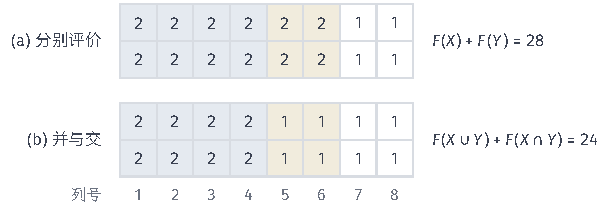
\includegraphics[width=103.258mm]{figures/01-basic-mathematics/04-graphs/tikz/c4-submodular-overlap-count/figure.pdf}
  \caption{覆盖函数上四值不等式的逐格计数，取$X=\{a,b\}$、$Y=\{b,c\}$。(a) 每格的数字是$X$与$Y$中覆盖它的组数，合计$F(X)+F(Y)$；(b) 每格的数字是$X\cup Y$与$X\cap Y=\{b\}$中覆盖它的组数，合计$F(X\cup Y)+F(X\cap Y)$。蓝底的第$1$至$4$列由公共部分覆盖，两边相同；黄底的第$5$、$6$列被$X$的$a$与$Y$的$c$分别覆盖而不被$b$覆盖，左边多计一次，四格合计正是差值$4$。}
  \label{fig:graph-setfn-submodular-overlap-count}
\end{figure}

\paragraph{割权的次模性}
割权按边累加，所以先看一条权为$w$的边$\{i,j\}$单独贡献的函数：它在$S$恰含$i,j$之一时取$w$，否则取$0$。对不是端点的元素，这条边的贡献不随它的加入而改变，增益为$0$。加入端点$i$时，若$j$已在集合中，这条边从跨越两侧变为两端同侧，增益为$-w$；若$j$不在集合中，这条边从两端同侧变为跨越两侧，增益为$+w$。

现在取$A\subseteq B$、$i\notin B$，按$j$的归属分三种情形比较两个增益，见图~\ref{fig:graph-setfn-cut-submodular-cases}。若$j\in A$，则$j$也在$B$中，两个增益都是$-w$；若$j\in B\setminus A$，则$\Delta(i\mid A)=+w$而$\Delta(i\mid B)=-w$；若$j\notin B$，两个增益都是$+w$。三种情形都满足$\Delta(i\mid A)\geq\Delta(i\mid B)$；待加入的元素不是这条边的端点时，两个增益都是$0$，不等式也成立。所以单条边的贡献是次模的。

由次模函数之和仍是次模函数，$\operatorname{cut}$作为各边贡献之和也是次模的。边权非负在这里是必要的：若某条边的权为负，第二种情形的不等号就反向了。

\begin{figure}[!htb]
  \centering
  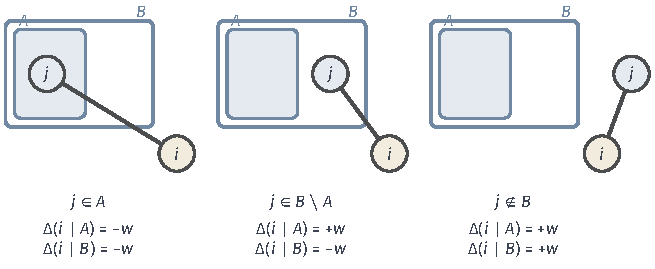
\includegraphics[width=110.723mm]{figures/01-basic-mathematics/04-graphs/tikz/c4-cut-submodular-cases/figure.pdf}
  \caption{割权函数次模性的逐边验证。固定一条权为$w\geq0$的边$\{i,j\}$，已选集合$A\subseteq B$（内框为$A$，外框为$B$），待加入的端点$i$（黄色）不在$B$中。按另一端点$j$的位置分三种情形：$j\in A$时两个增益都是$-w$；$j\in B\setminus A$时$A$上增益为$+w$、$B$上增益为$-w$；$j\notin B$时两个增益都是$+w$。每种情形都有$\Delta(i\mid A)\geq\Delta(i\mid B)$。}
  \label{fig:graph-setfn-cut-submodular-cases}
\end{figure}

\subsection{性质之间的关系}
\label{sec:graph-setfn-property-relations}

次模与单调互不蕴含。割权常常随集合增大而下降：$\operatorname{cut}(\varnothing)=\operatorname{cut}(V)=0$，而中间的子集可以有正的割权。图~\ref{fig:graph-setfn-property-counterexamples}(b)是只有一条权$1$的边的情形，割权依次为$0,1,1,0$，从单元素集到$\{1,2\}$时下降，所以次模函数不必单调。

反方向，图~\ref{fig:graph-setfn-property-counterexamples}(a)的函数
\[
  F(S)=\max\bigl\{3\,\mathbb I\{\{1,2\}\subseteq S\},\ \mathbb I\{3\in S\}\bigr\}
\]
是单调的，但$\Delta(2\mid\varnothing)=0<3=\Delta(2\mid\{1\})$，违反式~\eqref{eq:graph-setfn-diminishing-returns}，所以单调函数也不必次模。

\begin{figure}[!htb]
  \centering
  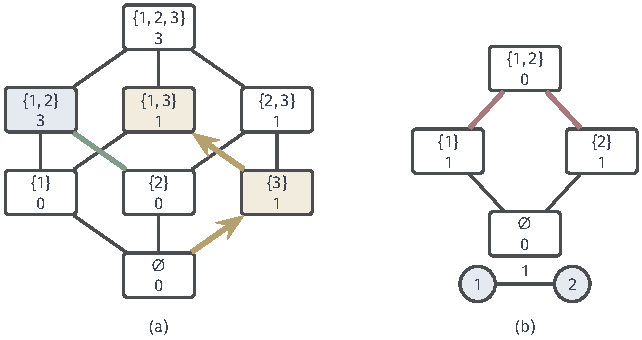
\includegraphics[width=108.687mm]{figures/01-basic-mathematics/04-graphs/tikz/c4-property-counterexamples/figure.pdf}
  \caption{单调性与次模性互不蕴含。每个框上行是子集，下行是函数值，连线连接只差一个元素的子集。(a) $F(S)=\max\{3\,\mathbb I\{\{1,2\}\subseteq S\},\mathbb I\{3\in S\}\}$：沿任一连线向上函数值不减，但绿色连线$\{2\}\to\{1,2\}$的增益$3$大于从空集加入$2$的增益$0$；黄色箭头是第~\ref{sec:graph-cardinality-selection}节贪心选择的路径，蓝色框是两元素时的最优集合。(b) 单条权$1$的边上的割权：次模，但红色连线上函数值从$1$降到$0$。}
  \label{fig:graph-setfn-property-counterexamples}
\end{figure}

\paragraph{超模函数}
把式~\eqref{eq:graph-setfn-diminishing-returns}的不等号反过来，即要求$\Delta(v\mid A)\leq\Delta(v\mid B)$，得到的函数称为\term{超模}函数（supermodular function）；等价地，$F$超模当且仅当$-F$次模。

超模描述的是协同：两个部件只有同时具备才能工作时，单独加入任何一个的增益都是$0$，在另一个已经存在时加入，增益才是正的。例如$F(S)=\mathbb I\{\{1,2\}\subseteq S\}$是超模的。

图~\ref{fig:graph-setfn-property-counterexamples}(a)的函数既不是次模也不是超模：元素$1,2$之间是协同的，而元素$3$与$\{1,2\}$之间是替代的，$\Delta(3\mid\varnothing)=1>0=\Delta(3\mid\{1,2\})$。模函数的增益恒为$w_v$，与已选集合无关，同时满足两个方向的不等式，所以它既是次模的也是超模的。

但同时次模和超模并不带来单调：由第~\ref{sec:graph-setfn-modularity}小节，模函数是否单调只取决于权重的符号。例如二元底集上取$c_0=0$、$w_1=1$、$w_2=-1$，则$F(\{1,2\})=0<1=F(\{1\})$，这个模函数既次模又超模，却不单调。

\paragraph{性质对照}
表~\ref{tab:graph-setfn-property-summary}汇总本节的函数（割权取图~\ref{fig:graph-setfn-property-counterexamples}(b)的单边图）。

表中尚未直接核对的几项如下：
\begin{itemize}
  \item 覆盖量：$\Delta(c\mid\varnothing)=8>4=\Delta(c\mid\{a\})$，增益随已选集合变小，所以不是超模的。
  \item 单边割权：$\Delta(1\mid\varnothing)=1>-1=\Delta(1\mid\{2\})$，所以不是超模的；$\operatorname{cut}(\{1\})+\operatorname{cut}(\{2\})=2\neq0=\operatorname{cut}(\{1,2\})+\operatorname{cut}(\varnothing)$，所以不是模函数。
  \item 净收益：它是次模函数$F$加上模函数$-c$，仍为次模。若它是模函数或超模函数，再加回模函数$c$，$F$也会是模函数或超模函数，与前两行矛盾；所以它同$F$一样既不是模函数也不是超模的。
  \item $\mathbb I\{\{1,2\}\subseteq S\}$：加入一个元素的增益只在另一元素已选时为$1$，随已选集合只增不减，所以是超模的；$\Delta(2\mid\varnothing)=0<1=\Delta(2\mid\{1\})$说明它不是次模的。
\end{itemize}

四种性质可以各种方式组合出现。所以后两章的算法保证都同时写明目标方向、函数是否单调、是否次模以及约束；只凭“次模”二字，不能决定采用哪种方法。

\begin{table}[!htb]
  \centering
  \caption{本节各函数的性质。“是”“否”均已在正文中由定义、判别式或反例核对；模函数同时满足次模与超模的不等式。}
  \label{tab:graph-setfn-property-summary}
  \small
  \begin{tabular}{@{}lcccc@{}}
    \toprule
    函数 & 单调 & 模 & 次模 & 超模 \\
    \midrule
    总成本$c$ & 是 & 是 & 是 & 是 \\
    覆盖量$F$ & 是 & 否 & 是 & 否 \\
    割权$\operatorname{cut}$ & 否 & 否 & 是 & 否 \\
    净收益$F-c$ & 否 & 否 & 是 & 否 \\
    $\mathbb I\{\{1,2\}\subseteq S\}$ & 是 & 否 & 否 & 是 \\
    图~\ref{fig:graph-setfn-property-counterexamples}(a)的函数 & 是 & 否 & 否 & 否 \\
    \bottomrule
  \end{tabular}
\end{table}

% 第8章第3节：子集累计与 Möbius 反演（子集格与累计；Möbius 反演及四元素算例；反演的计算：逐元素差分；有限偏序集上的推广）。

\section{子集累计与 Möbius 反演}
\label{sec:comb-cumulative-inversion}

设想每个课程组合有一个总得分：单门课各有自己的贡献，某两门课同时选又会产生额外的配合效果，配合也可能是负的。能观察到的是每个组合的总得分，想知道的却是每个组合\emph{自身}贡献了多少。

卷一计数中的容斥原理由各交集的大小恢复并集的大小，这里做的是同一类“由累计量恢复局部量”的事，只是对象换成了一般的数值。本节只用有限求和与包含关系，不依赖上一节的单调或次模假设，也不是后面选择算法的前提。

\subsection{子集格与累计}
\label{sec:graph-setfn-subset-lattice}

累计沿包含关系进行，所以先把包含关系画出来。包含关系是幂集上的偏序：每个集合包含自身；$S\subseteq T$与$T\subseteq S$同时成立时$S=T$；包含关系可以传递。有限集合$V$的全部子集连同包含关系称为$V$的\term{子集格}（subset lattice）：两个子集的交是它们最大的公共子集，并是包含两者的最小集合。

图~\ref{fig:comb-mobius-cumulative-local}按元素个数自下而上分层画出$V_0=\{1,2,3,4\}$的子集格，每条连线连接只差一个元素的两个子集，沿连线向上一步就是加入一个元素。图~\ref{fig:graph-setfn-subset-binary-cube}中的立方体正是三元底集的子集格。

从$S$出发沿连线一路向下能到达的子集，恰好是$S$的全部子集，例如从$\{1,3\}$向下只能到达$\{1\}$、$\{3\}$和空集。累计值就沿这些向下的路径收集贡献。

\begin{figure}[!htb]
  \centering
  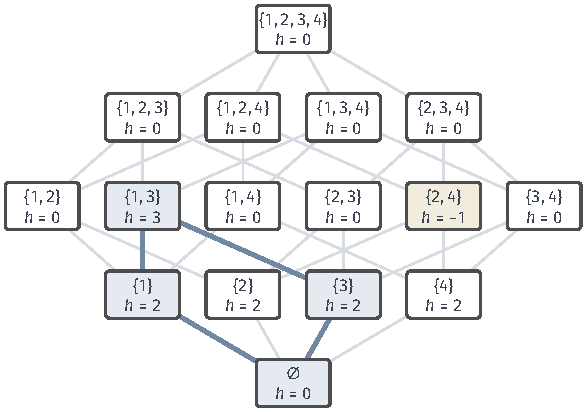
\includegraphics[width=99.187mm]{figures/01-basic-mathematics/04-graphs/tikz/c4-subset-lattice-cumulative/figure.pdf}
  \caption{四元素集合$V_0=\{1,2,3,4\}$的子集格与各子集自身的贡献$h$。子集按元素个数自下而上分层，连线连接只差一个元素的两个子集；框内上行为子集，下行为教学设定的贡献。蓝色标出$\{1,3\}$及其全部子集，它们的贡献相加得到累计值$g(\{1,3\})=0+2+2+3=7$；黄色框$\{2,4\}$的自身贡献为负。}
  \label{fig:comb-mobius-cumulative-local}
\end{figure}

\paragraph{自身贡献与累计值}
给每个子集$T$指定一个实数$h(T)$，表示$T$作为整体\emph{自身}带来的贡献：单元素集的贡献是单门课的得分，二元集的贡献是两门课在各自得分之外的配合效果，依此类推。$S$的累计值收集它的全部子集的贡献：
\begin{equation}
  g(S)=\sum_{T\subseteq S}h(T).
  \label{eq:comb-zeta-transform}
\end{equation}
$g$与$h$都是$V$上的集合函数。累计不只相加单元素的贡献，$S$内部更大子集的配合贡献也计入其中。

图~\ref{fig:comb-mobius-cumulative-local}的教学设定让四个单项各贡献$2$，$\{1,3\}$另有配合贡献$3$，$\{2,4\}$另有配合贡献$-1$，其余子集（包括空集和全部三元、四元子集）的贡献为$0$。于是
\[
  g(\{1,3\})=h(\varnothing)+h(\{1\})+h(\{3\})+h(\{1,3\})=0+2+2+3=7,
\]
而两个单项的累计值之和只有$g(\{1\})+g(\{3\})=4$，多出的$3$正是$\{1,3\}$自身的贡献。

反演处理相反方向的问题：已知全部$2^n$个累计值$g(S)$，求全部$2^n$个自身贡献$h(S)$，使它们按式~\eqref{eq:comb-zeta-transform}累计后恰好给出已知的$g$。需要回答的是这样的$h$是否存在、是否唯一，以及怎样算出来。

\subsection{Möbius 反演}
\label{sec:graph-setfn-mobius-inversion}

先看一列数的情形。若$g_k=h_1+\cdots+h_k$是前缀和，恢复$h_k$只需相邻两项相减：
\[
  h_k=g_k-g_{k-1}.
\]
子集格上的累计也是一种“前缀和”，只是$S$的下方不止一个紧邻的子集，而有$|S|$个$S\setminus\{i\}$，每个元素给出一个相减的方向。只沿一个方向相减还不够，各个方向的差会把某些贡献重复减去，需要再加回来。

两元素的情形可以完整写出。$g(\{1,3\})$包含$h(\varnothing)$、$h(\{1\})$、$h(\{3\})$和$h(\{1,3\})$四项。为了只留下$h(\{1,3\})$，先减去
\[
  g(\{1\})=h(\varnothing)+h(\{1\}),\qquad g(\{3\})=h(\varnothing)+h(\{3\}),
\]
两个单项贡献被去掉，但$h(\varnothing)$被多减了一次，再加回$g(\varnothing)=h(\varnothing)$，剩下的恰是
\[
  h(\{1,3\})=g(\{1,3\})-g(\{1\})-g(\{3\})+g(\varnothing).
\]

表~\ref{tab:graph-setfn-mobius-cancellation}逐项记录四个累计值各含哪些贡献、带什么符号：按列相加，$h(\varnothing)$、$h(\{1\})$、$h(\{3\})$的系数都抵消为$0$，只有$h(\{1,3\})$留下系数$1$。

同一个式子也是两次相邻差：
\[
  h(\{1,3\})=\bigl(g(\{1,3\})-g(\{3\})\bigr)-\bigl(g(\{1\})-g(\varnothing)\bigr),
\]
两个括号各沿“加入元素$1$”的方向相减，括号之间再沿“加入元素$3$”的方向相减。展开后，每个$g(T)$的符号由$T$比$S$少几个元素决定，少一个变一次号。一般情形的公式正是这样，称为\term{Möbius反演}（Möbius inversion）。

\begin{table}[!htb]
  \centering
  \begin{tabular}{@{}lcccc@{}}
    \toprule
    & $h(\varnothing)$ & $h(\{1\})$ & $h(\{3\})$ & $h(\{1,3\})$ \\
    \midrule
    $+g(\{1,3\})$ & $+1$ & $+1$ & $+1$ & $+1$ \\
    $-g(\{1\})$ & $-1$ & $-1$ & & \\
    $-g(\{3\})$ & $-1$ & & $-1$ & \\
    $+g(\varnothing)$ & $+1$ & & & \\
    \midrule
    合计 & $0$ & $0$ & $0$ & $1$ \\
    \bottomrule
  \end{tabular}
  \caption{$h(\{1,3\})=g(\{1,3\})-g(\{1\})-g(\{3\})+g(\varnothing)$中各项的抵消。每行把一个累计值按式~\eqref{eq:comb-zeta-transform}展开，记下各贡献的系数（已乘上该累计值前的符号），空白为$0$；末行按列相加。}
  \label{tab:graph-setfn-mobius-cancellation}
\end{table}

\begin{theorem}[子集格上的 Möbius 反演]
\label{thm:comb-mobius-inversion}
设$V$为有限集合，$g,h:\mathcal P(V)\to\mathbb R$。若对每个$S\subseteq V$式~\eqref{eq:comb-zeta-transform}成立，则对每个$S\subseteq V$有
\begin{equation}
  h(S)=\sum_{T\subseteq S}(-1)^{|S|-|T|}g(T).
  \label{eq:comb-mobius-inversion}
\end{equation}
反过来，若对每个$S$式~\eqref{eq:comb-mobius-inversion}成立，则式~\eqref{eq:comb-zeta-transform}也对每个$S$成立。
\end{theorem}

\begin{proof}
把式~\eqref{eq:comb-zeta-transform}代入式~\eqref{eq:comb-mobius-inversion}右侧，得到对全部满足$R\subseteq T\subseteq S$的集合对$(R,T)$的双重和。先固定$T$再取$R$，与先固定$R$再取$T$，遍历的是同一批有限个集合对；有限和只是把这些项全部相加，与分组次序无关，所以可以交换求和次序：
\[
  \begin{aligned}
  &\sum_{T\subseteq S}(-1)^{|S|-|T|}\sum_{R\subseteq T}h(R)\\
  &\qquad=\sum_{R\subseteq S}h(R)\sum_{T:\,R\subseteq T\subseteq S}(-1)^{|S|-|T|}.
  \end{aligned}
\]
固定$R$后，满足$R\subseteq T\subseteq S$的$T$由$S\setminus R$中哪些元素被加入决定，即$T=R\cup D$，$D\subseteq S\setminus R$任意，且$|S|-|T|=|S\setminus R|-|D|$。记$q=|S\setminus R|$，按$|D|=j$分组，大小为$j$的$D$有$\binom qj$个，所以内层和等于
\[
  \begin{aligned}
  \sum_{j=0}^{q}\binom qj(-1)^{q-j}&=(-1)^q\sum_{j=0}^{q}(-1)^j\binom qj\\
  &=\begin{cases}1,&q=0,\\0,&q\geq1,\end{cases}
  \end{aligned}
\]
最后一步用组合数的交错和：$q\geq1$时，$q$元集合中偶数大小的子集与奇数大小的子集一样多（固定一个元素，加入或删去它就把两类一一配对），所以$\sum_{j=0}^{q}(-1)^j\binom qj=0$。

内层和只在$R=S$时为$1$，在$R$是$S$的真子集时为$0$，所以真子集上的贡献全部抵消，右侧只剩$h(S)$。表~\ref{tab:graph-setfn-mobius-cancellation}的各列合计正是$S=\{1,3\}$时的这些内层和。

反方向同样直接核对。由式~\eqref{eq:comb-mobius-inversion}给出$h$，代入$\sum_{T\subseteq S}h(T)$并交换求和次序，
\[
  \sum_{T\subseteq S}h(T)=\sum_{R\subseteq S}g(R)\sum_{T:\,R\subseteq T\subseteq S}(-1)^{|T|-|R|}.
\]
仍写$T=R\cup D$，内层和等于$\sum_{j=0}^{q}(-1)^j\binom qj$，它在$R=S$时只有$D=\varnothing$一项而等于$1$，在$R\neq S$时为$0$。所以右侧等于$g(S)$。
\end{proof}

定理回答了存在与唯一的问题。对任意给定的$g$，按式~\eqref{eq:comb-mobius-inversion}定义的$h$累计后恰好回到$g$，所以所求的$h$存在；而任何满足式~\eqref{eq:comb-zeta-transform}的$h$都必须等于式~\eqref{eq:comb-mobius-inversion}的右侧，所以它是唯一的。

式~\eqref{eq:comb-zeta-transform}与式~\eqref{eq:comb-mobius-inversion}是一对互逆的变换：从贡献到累计，再从累计回到贡献，不丢失任何信息。

证明中起作用的是组合数的交错和为零，这与容斥原理相同；区别在于容斥使并集中每个元素恰计一次，反演只保留指定子集自身的贡献。

\paragraph{四元素算例}
仍用指示函数$\mathbb I\{\cdot\}$，沿用图~\ref{fig:comb-mobius-cumulative-local}的设定，累计值可以写成
\[
  g(S)=2|S|+3\,\mathbb I\{\{1,3\}\subseteq S\}-\mathbb I\{\{2,4\}\subseteq S\}.
\]
其中$2|S|$收集$S$中各单项的贡献，后两项在$S$包含$\{1,3\}$或$\{2,4\}$时计入相应的配合贡献。表~\ref{tab:comb-four-element-mobius}列出全部$16$个累计值，以及只用这些累计值按式~\eqref{eq:comb-mobius-inversion}恢复的贡献。

\begin{table}[!htb]
  \centering
  \begin{tabular}{ccc@{\qquad}ccc}
    \toprule
    $S$ & $g(S)$ & $h(S)$ & $S$ & $g(S)$ & $h(S)$ \\
    \midrule
    $\varnothing$ & $0$ & $0$ & $\{2,3\}$ & $4$ & $0$ \\
    $\{1\}$ & $2$ & $2$ & $\{2,4\}$ & $3$ & $-1$ \\
    $\{2\}$ & $2$ & $2$ & $\{3,4\}$ & $4$ & $0$ \\
    $\{3\}$ & $2$ & $2$ & $\{1,2,3\}$ & $9$ & $0$ \\
    $\{4\}$ & $2$ & $2$ & $\{1,2,4\}$ & $5$ & $0$ \\
    $\{1,2\}$ & $4$ & $0$ & $\{1,3,4\}$ & $9$ & $0$ \\
    $\{1,3\}$ & $7$ & $3$ & $\{2,3,4\}$ & $5$ & $0$ \\
    $\{1,4\}$ & $4$ & $0$ & $V_0$ & $10$ & $0$ \\
    \bottomrule
  \end{tabular}
  \caption{四元素子集格上的累计值$g$与由式~\eqref{eq:comb-mobius-inversion}恢复的自身贡献$h$。恢复结果与教学设定一致：四个单项各为$2$，$\{1,3\}$为$3$，$\{2,4\}$为$-1$，其余子集（包括全部三元子集和$V_0$）均为$0$。}
  \label{tab:comb-four-element-mobius}
\end{table}

逐个套用公式，两个二元子集的贡献按前面的四项公式恢复：
\[
  h(\{1,3\})=7-2-2+0=3,\qquad h(\{2,4\})=3-2-2+0=-1.
\]

三元子集要用到八个累计值。对$S=\{1,2,3\}$，按子集大小依次取三元、二元、一元和空集项，
\[
  h(\{1,2,3\})=9-(4+7+4)+(2+2+2)-0=0.
\]
虽然$\{1,2,3\}$包含有配合效果的$\{1,3\}$，它的累计值$9$也大于三个单项之和$6$，但多出的$3$已经由$h(\{1,3\})$解释，三门课之间没有新的整体效果，所以三元贡献为$0$。

$\{1,3,4\}$也是如此：$g=9$，恢复出$h=0$。其余两个三元子集同样得到$0$，例如
\[
  h(\{2,3,4\})=5-(4+3+4)+(2+2+2)-0=0,
\]
其中$-1$的配合贡献已由$h(\{2,4\})$解释。反演还允许贡献为负，$h(\{2,4\})=-1$就是一例。

\subsection{反演的计算}
\label{sec:graph-setfn-mobius-computation}

\subsubsection{问题与思路}

输入是全部$2^n$个累计值，输出是全部$2^n$个自身贡献。直接套用式~\eqref{eq:comb-mobius-inversion}，计算$h(S)$要读取$S$的全部$2^{|S|}$个子集上的累计值。

另一种做法是由式~\eqref{eq:comb-zeta-transform}移项逐个求解：
\[
  h(S)=g(S)-\sum_{T\subsetneq S}h(T).
\]
从$h(\varnothing)=g(\varnothing)$出发，按元素个数从小到大计算，算到$S$时它的全部真子集的$h$都已求出。在四元素算例中，先得到$h(\varnothing)=0$和单项贡献$2$，再得二元贡献，例如
\[
  h(\{1,3\})=7-(0+2+2)=3,
\]
最后得到三元贡献，例如
\[
  h(\{1,2,3\})=9-(0+2+2+2+0+3+0)=0.
\]

这种递推同样要对每个$S$遍历它的全部子集。$k$元子集有$\binom nk$个，各有$2^k$个子集，所以由二项式定理，两种做法读取的项数都是
\[
  \sum_{k=0}^{n}\binom nk2^k=3^n.
\]
两种做法的共同瓶颈是每个$S$都要单独遍历它的全部子集。

上一小节把单个值$h(\{1,3\})$写成了两次相邻差，这提示可以按元素而不是按子集组织计算。式~\eqref{eq:comb-mobius-inversion}中的符号可以按元素拆开：对$T\subseteq S$，$(-1)^{|S|-|T|}$是$S\setminus T$中每个元素各贡献一个$-1$的乘积。于是交错和可以一个元素一个元素地做：先对全部子集沿“加入元素$1$”的方向取相邻差，再在结果上沿元素$2$的方向取差，依此类推。

每个元素只处理一轮，一轮对$2^{n-1}$对相邻子集各做一次减法，不再为每个$S$单独遍历它的子集。这种做法称为逐元素差分。

\subsubsection{算法实现}

元素的编号$1,\ldots,n$与子集在数组中的位置在开始前确定，运行中不再改变，所以不把它们计入算法的状态。

\paragraph{子集数组的数据结构}
数组以子集为下标。沿用第~\ref{sec:graph-setfn-binary-vectors}小节的指示向量，把$S$的指示向量$(x_1,\ldots,x_n)$读成二进制数$\sum_{i=1}^{n}x_i2^{i-1}$，作为$S$在长度为$2^n$的数组中的位置。$S$含元素$i$，当且仅当这个数从低位数起的第$i$位为$1$；这时$S\setminus\{i\}$的位置是它减去$2^{i-1}$。例如$n=3$时$\{1,3\}$的位置是$101_2=5$，$\{1,3\}\setminus\{1\}=\{3\}$的位置是$5-1=4$。

依次扫描位置$0,1,\ldots,2^n-1$，挑出第$i$位为$1$的位置，就把含$i$的子集各访问一次，每次用一次减法找到$S\setminus\{i\}$。

\paragraph{逐元素差分的实现}
算法维护两项状态：
\begin{itemize}
  \item 数组$a(\cdot)$：以子集为下标，长度为$2^n$，初值$a(S)=g(S)$；
  \item 当前元素$i$：本轮处理的元素，初值为$1$。
\end{itemize}
第$i$轮按子集是否含$i$分别处理，处理完令$i\gets i+1$：
\begin{itemize}
  \item 含$i$的子集$S$：令$a(S)\gets a(S)-a(S\setminus\{i\})$；
  \item 不含$i$的子集：保持不变。
\end{itemize}
本轮读取的$a(S\setminus\{i\})$所在的子集不含$i$，本轮不会被修改，所以更新可以原地进行，不需要另存上一轮的数组。处理完元素$n$后停止，输出$a$。在子集格上看，第$i$轮只沿“加入元素$i$”方向的连线做差，图~\ref{fig:graph-setfn-subset-binary-cube}中同色的一组边就是一轮读取的方向。

\begin{algorithm}[逐元素差分]
\label{alg:graph-setfn-mobius-coordinate}
输入：底集$V=\{1,\ldots,n\}$上的全部累计值$g(S)$。输出：全部自身贡献$h(S)$。
\begin{enumerate}
  \item 对每个$S\subseteq V$置$a(S)=g(S)$；令$i=1$。
  \item 对每个含$i$的子集$S$，置$a(S)=a(S)-a(S\setminus\{i\})$；不含$i$的子集不变。
  \item 若$i<n$，令$i\gets i+1$并回到第2步；否则输出$h(S)=a(S)$。
\end{enumerate}
\end{algorithm}

\paragraph{执行过程}
先在三元子集格$\{1,2,3\}$上执行。四元素设定限制到$\{1,2,3\}$的子集上，仍是同一组累计值与贡献，因为$g(S)$和$h(S)$只读取$S$的子集。

初始数组就是累计值：
\[
  \begin{gathered}
  a(\varnothing)=0,\qquad a(\{1\})=a(\{2\})=a(\{3\})=2,\\
  a(\{1,2\})=4,\quad a(\{1,3\})=7,\quad a(\{2,3\})=4,\quad a(\{1,2,3\})=9.
  \end{gathered}
\]

\begin{BookInlineFigure}
  \centering
  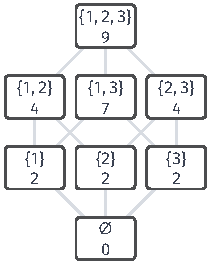
\includegraphics[width=35.736mm]{figures/03-graphs/03-set-functions-and-subset-selection/tikz/reading-steps/mobius-round-0.pdf}
  \caption{逐元素差分的初始状态：每个框的上行是子集$S$，下行是累计值$g(S)$。本例取四元素设定限制到$\{1,2,3\}$的值。}
  \label{fig:graph-setfn-mobius-coordinate-rounds}
\end{BookInlineFigure}

每轮只改动含被处理元素的四个子集：
处理元素$1$：$\{1\}$为$2-0=2$，$\{1,2\}$为$4-2=2$，$\{1,3\}$为$7-2=5$，$\{1,2,3\}$为$9-4=5$。
\begin{BookInlineFigure}
  \centering
  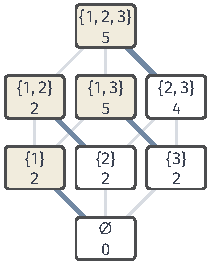
\includegraphics[width=35.736mm]{figures/03-graphs/03-set-functions-and-subset-selection/tikz/reading-steps/mobius-round-1.pdf}
  \caption{处理元素$1$后的数组。黄色子集含$1$；蓝色粗线连接该子集与本轮读取的$S\setminus\{1\}$，框内下行已写入相减后的值。}
  \label{fig:graph-setfn-mobius-coordinate-rounds-1}
\end{BookInlineFigure}

处理元素$2$：$\{2\}$为$2-0=2$，$\{1,2\}$为$2-2=0$，$\{2,3\}$为$4-2=2$，$\{1,2,3\}$为$5-5=0$。
\begin{BookInlineFigure}
  \centering
  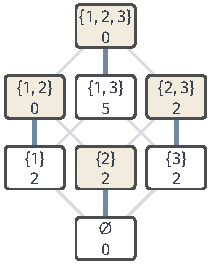
\includegraphics[width=35.736mm]{figures/03-graphs/03-set-functions-and-subset-selection/tikz/reading-steps/mobius-round-2.pdf}
  \caption{处理元素$2$后的数组。本轮只沿蓝色粗线做差，改写含$2$的四个黄色子集；其余值保持不变。}
  \label{fig:graph-setfn-mobius-coordinate-rounds-2}
\end{BookInlineFigure}

处理元素$3$：$\{3\}$为$2-0=2$，$\{1,3\}$为$5-2=3$，$\{2,3\}$为$2-2=0$，$\{1,2,3\}$为$0-0=0$。
\begin{BookInlineFigure}
  \centering
  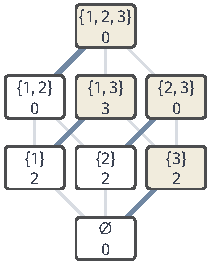
\includegraphics[width=35.736mm]{figures/03-graphs/03-set-functions-and-subset-selection/tikz/reading-steps/mobius-round-3.pdf}
  \caption{处理元素$3$后的数组，即自身贡献$h$。此时$h(\{1,3\})=3$，单项贡献各为$2$，其余值为$0$。}
  \label{fig:graph-setfn-mobius-coordinate-rounds-3}
\end{BookInlineFigure}

最终数组就是$h$：单项各为$2$，$h(\{1,3\})=3$，其余为$0$。

$\{1,3\}$的值$7\to5\to5\to3$正是上一小节的两次相邻差：处理元素$1$时减去$g(\{3\})$，处理元素$3$时减去已经差分过的$a(\{1\})=g(\{1\})-g(\varnothing)$。图~\ref{fig:graph-setfn-mobius-coordinate-rounds-1}至图~\ref{fig:graph-setfn-mobius-coordinate-rounds-3}分别给出各轮结束后的状态。


四元素算例照样做四轮，每轮改动含$i$的$8$个子集，最后的数组与表~\ref{tab:comb-four-element-mobius}中的$h$逐项一致。例如$\{2,4\}$依次为$3,3,1,1,-1$：处理元素$2$时减去$a(\{4\})=2$，处理元素$4$时减去当前的$a(\{2\})=2$。中间各轮的数组只是部分差分，只有最后一轮之后才是$h$。

\subsubsection{算法分析}

\paragraph{正确性}
上面按元素拆分符号的说法，可以由一个不变式精确表达。记$[i]=\{1,\ldots,i\}$。断言：处理完元素$1,\ldots,i$后，
\[
  a(S)=\sum_{\substack{T\subseteq S\\ T\setminus[i]=S\setminus[i]}}(-1)^{|S|-|T|}g(T),
\]
即只对那些与$S$在元素$i+1,\ldots,n$上一致的子集$T$做交错求和。$i=0$时条件迫使$T=S$，右侧就是$g(S)$，与初始化一致。

设断言对$i$成立，看第$i+1$轮。若$i+1\notin S$，$a(S)$不变；而$S$的子集都不含$i+1$，“在$i+1,\ldots,n$上一致”与“在$i+2,\ldots,n$上一致”是同一个条件，断言对$i+1$成立。

若$i+1\in S$，新值是
\[
  a(S)-a(S\setminus\{i+1\}).
\]
前一项求和的$T$与$S$在$i+1,\ldots,n$上一致，因而含$i+1$；后一项求和的$T$与$S\setminus\{i+1\}$一致，因而不含$i+1$，符号$(-1)^{|S|-1-|T|}$再乘以$-1$变成$(-1)^{|S|-|T|}$。两组$T$合起来，恰是与$S$在$i+2,\ldots,n$上一致的全部子集，断言对$i+1$成立。

取$i=n$，条件不再限制$T$，右侧正是式~\eqref{eq:comb-mobius-inversion}，所以输出就是$h$。

\paragraph{复杂度}
逐元素差分每轮做$2^{n-1}$次减法，共$n2^{n-1}$次；按上面的数据结构，每次找到$S\setminus\{i\}$只需一次整数减法，原地更新只用长度为$2^n$的数组。逐个套用公式与按子集大小递推都需要$3^n$次运算，四元素算例中是$32$次对$81$次。

不过输入本身已有$2^n$个数，三种方式的运算量都随$n$指数增长。逐元素差分降低的是指数的底，从$3$降到$2$，并没有使计算摆脱指数规模。

\paragraph{累计方向}
把每一轮的减号换成加号、从$a=h$出发做$n$轮，同样的归纳（不变式中的符号$(-1)^{|S|-|T|}$换成$1$，$g$换成$h$）说明得到的是累计值$g$。例如$\{1,3\}$由$3$经$3+2=5$、$5+2=7$回到$g(\{1,3\})$。所以累计和反演可以用同一套逐元素扫描完成，开销也相同。

\subsection{有限偏序集上的推广}
\label{sec:graph-setfn-poset-mobius}

反演公式中的系数$(-1)^{|S|-|T|}$只依赖两个子集的相对位置。同样的问题可以在任意有限偏序集$(X,\preceq)$上提出：给每个元素$y$一个数$h(y)$，沿下方累计得
\[
  g(x)=\sum_{y\preceq x}h(y),
\]
再问怎样由$g$恢复$h$。这时系数不再一律是$\pm1$，而由下面的函数确定。

\begin{definition}[Möbius 函数]
\label{def:graph-setfn-mobius-function}
设$(X,\preceq)$是有限偏序集，记$y\prec x$表示$y\preceq x$且$y\neq x$。偏序集的\term{Möbius函数}（Möbius function）$\mu$对满足$y\preceq x$的元素对定义为
\begin{equation}
  \mu(y,y)=1,\qquad \mu(y,x)=-\sum_{z:\,y\preceq z\prec x}\mu(y,z)\quad(y\prec x),
  \label{eq:graph-setfn-mobius-function-def}
\end{equation}
对不满足$y\preceq x$的元素对取$\mu(y,x)=0$。
\end{definition}

定义固定区间的下端$y$，从对角值$\mu(y,y)=1$出发向上递推：算$\mu(y,x)$时只用到区间$\{z:y\preceq z\prec x\}$上已经算出的值，而有限偏序集保证递推在有限步内完成。递推式移项后写成
\begin{equation}
  \sum_{z:\,y\preceq z\preceq x}\mu(y,z)=0\qquad(y\prec x),
  \label{eq:graph-setfn-mobius-function-sum}
\end{equation}
即每个非平凡区间上的系数之和为零；$y=x$时这个和是$\mu(y,y)=1$。

这一抵消性质足以完成反演，论证分两步。先定义
\[
  \tilde h(x)=\sum_{y\preceq x}\mu(y,x)g(y),
\]
并验证它累计后回到$g$。对任意$s\in X$，交换有限和的次序，
\[
  \begin{aligned}
  \sum_{x\preceq s}\tilde h(x)&=\sum_{x\preceq s}\sum_{y\preceq x}\mu(y,x)g(y)\\
  &=\sum_{y\preceq s}g(y)\sum_{x:\,y\preceq x\preceq s}\mu(y,x).
  \end{aligned}
\]
由式~\eqref{eq:graph-setfn-mobius-function-sum}，内层和在$y\prec s$时为$0$，在$y=s$时为$1$，所以右侧等于$g(s)$。

再说明满足累计式的$h$只有一个。累计式可以写成
\[
  h(x)=g(x)-\sum_{y\prec x}h(y),
\]
右侧只用到严格位于$x$下方的元素。把有限偏序集的元素排成一列，使每个元素都排在它上方的元素之前（例如反复取出当前剩余元素中的一个极小元），按这个次序逐个计算，$h$的每个值都被$g$唯一确定。$\tilde h$也满足累计式，所以$h=\tilde h$，即
\begin{equation}
  h(x)=\sum_{y\preceq x}\mu(y,x)g(y).
  \label{eq:graph-setfn-poset-mobius-inversion}
\end{equation}

在子集格上，$\mu(T,S)=(-1)^{|S|-|T|}$满足这个递推：对$T\subsetneq S$，记$q=|S\setminus T|\geq1$，
\[
  \sum_{R:\,T\subseteq R\subseteq S}(-1)^{|R|-|T|}=\sum_{j=0}^{q}(-1)^j\binom qj=0.
\]
由于递推从$\mu(T,T)=1$出发唯一确定全部值，子集格上的Möbius函数就是$(-1)^{|S|-|T|}$，只取$\pm1$，式~\eqref{eq:comb-mobius-inversion}是一般反演式的特例。

\paragraph{整除偏序}
图~\ref{fig:graph-setfn-mobius-divisors}是$12$的六个正因数在整除关系下的偏序。从$\mu(1,1)=1$出发，先得$\mu(1,2)=\mu(1,3)=-1$。区间$\{1,2,4\}$是一条链，区间$\{1,2,3,6\}$与两元素的子集格形状相同，从$1$到$12$的区间含全部六个因数。按定义逐个递推，
\[
  \begin{aligned}
  \mu(1,4)&=-(1-1)=0,\\
  \mu(1,6)&=-(1-1-1)=1,\\
  \mu(1,12)&=-(1-1-1+0+1)=0.
  \end{aligned}
\]
系数出现了$0$，说明一般偏序上的反演确实不同于子集格上的交错加减。

这一推广只是补充，后两章的选择算法都不以它为前提。

\begin{figure}[!htb]
  \centering
  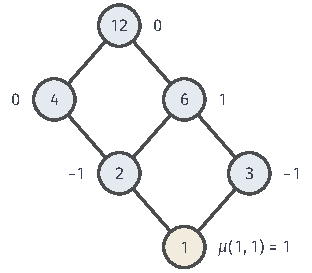
\includegraphics[width=52.613mm]{figures/01-basic-mathematics/04-graphs/tikz/c4-mobius-divisor-poset/figure.pdf}
  \caption{$12$的正因数在整除关系下的偏序，连线连接直接相邻的两个因数，下方整除上方。节点旁的数是$\mu(1,x)$，由$\mu(1,1)=1$（黄色节点）自下而上递推得到。链$1\mid2\mid4$上$\mu(1,4)=0$，与子集格同形的区间$\{1,2,3,6\}$上$\mu(1,6)=1$。}
  \label{fig:graph-setfn-mobius-divisors}
\end{figure}

\FloatBarrier
\section{本章小结}
\label{sec:set-functions-chapter-summary}

本章从传感器覆盖出发，把对整组选择的评价写成有限底集上的集合函数。底集可以是传感器，也可以是图的顶点或边，不必带图结构。$n$元底集的完整取值表有$2^n$项，所以函数通常由求值规则给出，算法的代价要分开计入求值次数和每次求值的开销。指示向量把子集换成零一向量，只换了索引方式，不带来可加性或局部分解。边际增益$\Delta(v\mid S)$是后面一切判别的基本量：它依赖已选集合，沿任一加入次序累加，总和等于两端函数值之差。

用边际增益可以分别回答三个问题。单调性问新增元素会不会降低评价，等价于全部边际增益非负；模性问每个元素的贡献是否固定，等价于四值等式，模函数恰是常数加固定权重之和；次模性问收益是否随已选集合增大而递减，在有限底集上与四值不等式等价。覆盖量与非负边权的割权是次模的典型例子，协同效应则给出超模函数。

这些性质互不蕴含。割权次模而不单调；$\max\{3\,\mathbb I\{\{1,2\}\subseteq S\},\mathbb I\{3\in S\}\}$中元素$1,2$只有同时选中才有大价值，它单调而不次模；模函数同时次模和超模，却可能因为负权重而不单调。归一化只是减去常数$F(\varnothing)$的约定，不改变任何边际增益。所以后面引用某种算法保证时，要逐项写明它需要哪些性质，不能只凭“次模”判断。

子集累计与Möbius反演回答另一个问题：由全部累计值恢复每个子集自身的贡献。反演按元素个数之差交替加减，依靠的是组合数交错和为零的抵消，它与累计互为逆变换，结果可以为负。这一问题只依赖有限求和与包含关系，不需要单调或次模。计算上，逐个套用公式和按子集大小递推都要$3^n$次运算，逐元素差分降到$n2^{n-1}$次，但仍随底集大小指数增长。一般有限偏序集上，Möbius函数由区间递推确定，子集格上的交替符号是它的特例。

下一章利用本章的边际增益和次模性，在基数或预算约束下最大化集合函数；第~\ref{chap:pairwise-binary-minimization}章再把一类可分解为一元项与成对项的次模函数化为割，精确求最小值。


\chapter{约束下的子集选择}
\label{chap:constrained-subset-selection}

上一章的传感器实例里，四个传感器合起来能覆盖全部$16$格。实际中名额或经费有限：只能装两个传感器时该装哪两个？各传感器价格不同、总经费固定时又该怎样选？这类问题在有限底集上最大化一个集合函数，同时限制所选子集的规模或总成本。小实例可以枚举全部可行子集，底集稍大时枚举就不可行，于是需要只看少量子集、又能说明结果离最优有多远的方法。

本章研究逐轮加入元素的贪心规则，分基数约束和预算约束两节。第~\ref{sec:graph-cardinality-selection}节在“至多选$k$个”的限制下每轮加入边际增益最大的元素，证明目标归一化、单调且次模时，所得值不低于最优值的$1-(1-1/k)^k$倍；同一节还说明次模性怎样让旧增益成为当前增益的上界，从而得到减少求值次数的惰性贪心。第~\ref{sec:graph-budget-selection}节让各元素占用不同的预算，把比较依据换成单位成本的增益，并用反例说明这一规则不能继承基数约束下的保证。

两节都要分清三件事：贪心规则本身对任何集合函数都能执行；惰性实现与普通贪心选出同样元素要靠次模性；比例保证则同时依赖归一化、单调、次模和约束的形式。本章使用上一章的边际增益、逐个加入的累计式和次模性的两种刻画。

% 第9章第1节：基数约束下的子集选择（问题与思路；算法实现；算法分析；惰性贪心）。

\section{基数约束下的子集选择}
\label{sec:graph-cardinality-selection}

回到传感器。只允许安装$k$个传感器时，应当选哪几个？枚举很快变得不可行，于是改为逐轮加入当前增益最大的元素。本节先给出这一规则及其实现，再证明目标归一化、单调且次模时所得值离最优值不远，最后利用次模性跳过大部分增益的重算。

\subsection{问题与思路}
\label{sec:graph-setfn-cardinality-problem}

设$V$是$n$元底集，$F$是$V$上的集合函数，整数$k$满足$0\leq k\leq n$。要求的是
\begin{equation}
  \max_{S\subseteq V,\ |S|\leq k}F(S).
  \label{eq:graph-setfn-cardinality-problem}
\end{equation}
“至多选$k$个”称为\term{基数约束}（cardinality constraint）。$F$通过求值规则给出：算法可以对任意子集询问$F$的值，每次询问计一次求值。计算成本因此同时取决于求值次数和每次求值的开销。算法输出一个至多含$k$个元素的集合，希望它的函数值尽量接近最优值。

对单调函数，“至多$k$个”与“恰好$k$个”给出同样的最优值。若某个最优集合不足$k$个元素，任意补入元素使它恰有$k$个，由单调性函数值不会下降，补足后的集合仍是最优的。非单调函数不能这样处理：补入的元素可能降低目标值，所以“至多”与“恰好”是两个不同的问题。

小底集可以枚举全部可行子集，所得的最优值是衡量其他方法的基准。在传感器实例中取$k=2$，可行子集有$\binom40+\binom41+\binom42=11$个。逐个读出覆盖量（第~\ref{sec:graph-setfn-definition}小节），最优值是$16$，最优集合唯一，为$\{b,c\}$；单元素中最好的是$\{a\}$，覆盖$10$格。

一般地，最优值是唯一的，最优集合却可能有多个并列；$k=3$时，$\{b,c\}$、$\{a,b,c\}$、$\{b,c,d\}$都覆盖全部$16$个格子，按“至多$3$个”的约束三者都是最优集合。

但枚举在规模稍大时就不可行。即使一次求值很便宜，$n=100$、$k=10$时，仅恰有$10$个元素的子集就有$\binom{100}{10}\approx1.7\times10^{13}$个。

只看少量子集的办法是逐步构造：从空集出发，每一轮在尚未选中的元素里挑当前增益最大的那个加入，选满$k$个为止。由式~\eqref{eq:graph-setfn-telescoping}，最终集合的函数值等于$F(\varnothing)$加上各轮增益之和，每一轮都让其中一项尽量大。

增益必须相对于已经选好的集合重新计算，只按初始增益排序一次是不够的。传感器实例中初始增益的次序是$a$为$10$，然后$b,c$并列为$8$；按编号取前两个得到$\{a,b\}$，只覆盖$12$格。选了$a$之后，$b$的增益从$8$降到$2$，$c$的增益从$8$降到$4$，排序已经改变。逐轮重算反映的正是已选元素造成的重叠。

\subsection{算法实现}
\label{sec:graph-setfn-greedy}

底集及其编号、整数$k$和求值规则都在运行前给定，运行中不变，不算状态。算法维护三项状态：
\begin{itemize}
  \item 已选集合$S$：初值为空集；
  \item 当前值$F(S)$：初值由一次求值得到$F(\varnothing)$，此后不另行求值，每轮加上选中元素的增益；
  \item 本轮增益：每个未选元素$v$相对于当前$S$的增益$\Delta(v\mid S)$，每轮开始时全部重新计算，不跨轮保留。
\end{itemize}
初始化只需一次求值，得到$F(\varnothing)$。每一轮做三件事：
\begin{itemize}
  \item 求增益：对每个$v\in V\setminus S$求值$F(S\cup\{v\})$，减去记录的当前值，得到$\Delta(v\mid S)$；
  \item 选择：取增益最大的元素$v$，增益相同时取编号最小者；
  \item 更新：令$F(S)\gets F(S)+\Delta(v\mid S)$，再令$S\gets S\cup\{v\}$。
\end{itemize}
$|S|=k$时停止，输出$S$。记第$t$轮选中的元素为$v_t$、结束时的集合为$S_t$，于是$S_0=\varnothing$，$S_t=S_{t-1}\cup\{v_t\}$。平局规则必须事先规定，否则同一输入可能得到不同输出，结果无法复核。

停止条件还有一种常用的变形：某一轮全部未选元素的增益都是$0$时提前停止，输出当前集合$S$。目标单调且次模时，这样做不损失函数值。

理由如下。对任意$T\subseteq V\setminus S$，把$T$的元素逐个加入$S$，由式~\eqref{eq:graph-setfn-telescoping}和次模性，每一步的增益不超过该元素相对于$S$的增益$0$，所以
\[
  F(S\cup T)\leq F(S);
\]
单调性又给出$F(S\cup T)\geq F(S)$，于是继续选满$k$个只会保持当前值。

只有单调性时，提前停止可能错过价值。单个元素的增益都是$0$，并不排除两个元素一起加入才产生价值。第~\ref{sec:graph-setfn-greedy-guarantee}小节末尾用到单调非次模函数
\[
  F(S)=\max\bigl\{3\,\mathbb I\{\{1,2\}\subseteq S\},\ \mathbb I\{3\in S\}\bigr\}.
\]
取$k=3$时，第$1$轮选$3$，第$2$轮元素$1,2$相对于$\{3\}$的增益都是$0$：提前停止得到$1$；继续选满则依次加入$1$、$2$，最后一步增益为$3$，得到$F(\{1,2,3\})=3$。

下面的算法与分析按选满$k$个书写。

\begin{algorithm}[基数约束下的边际增益贪心]
\label{alg:graph-setfn-greedy}
输入：有限底集$V$（元素已编号），整数$0\leq k\leq|V|$，单调非减集合函数$F$的求值规则。输出：至多含$k$个元素的集合。
\begin{enumerate}
  \item 令$S_0=\varnothing$，记录$F(S_0)$。
  \item 对$t=1,\ldots,k$：对每个$v\in V\setminus S_{t-1}$，求值$F(S_{t-1}\cup\{v\})$，得到$\Delta(v\mid S_{t-1})$；取增益最大的$v_t$，增益相同时取编号最小者；令$S_t=S_{t-1}\cup\{v_t\}$，$F(S_t)=F(S_{t-1})+\Delta(v_t\mid S_{t-1})$。
  \item 输出$S_k$。
\end{enumerate}
\end{algorithm}

\paragraph{执行过程}
在传感器实例上取$k=2$，按字母顺序编号。初始$S_0=\varnothing$，$F(S_0)=0$。
\begin{itemize}
  \item 第$1$轮：增益就是各传感器单独的覆盖量，$a,b,c,d$依次为$10,8,8,1$。选$a$，$S_1=\{a\}$，$F(S_1)=10$。
  \item 第$2$轮：相对于$\{a\}$重新计算。$b$只补上第$1$列的$2$格，$c$补上第$7$、$8$列的$4$格，$d$补上左上角$1$格，增益依次为$2,4,1$。选$c$，$S_2=\{a,c\}$，$F(S_2)=14$。
\end{itemize}
此时$|S|=k$，停止。图~\ref{fig:graph-setfn-greedy-rounds}把两轮增益画成条形，并与枚举最优集合$\{b,c\}$（$16$格）比较：贪心集合漏掉了第$1$列的两格。

\begin{figure}[!htb]
  \centering
  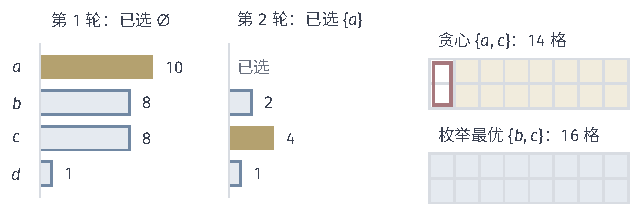
\includegraphics[width=107.177mm]{figures/01-basic-mathematics/04-graphs/tikz/c4-greedy-rounds-vs-optimum/figure.pdf}
  \caption{传感器实例上$k=2$的边际增益贪心。左侧两栏是两轮中各候选元素的当前增益，黄色条为该轮选中的元素；第$2$轮的增益相对于已选的$\{a\}$计算。右侧比较两个覆盖结果：贪心集合$\{a,c\}$（黄色）漏掉第$1$列两格（红框），枚举最优集合$\{b,c\}$（蓝色）覆盖全部$16$格。}
  \label{fig:graph-setfn-greedy-rounds}
\end{figure}

\subsection{算法分析}
\label{sec:graph-setfn-greedy-guarantee}

\paragraph{可行性}
算法每一轮恰好加入一个尚未选中的元素，执行$k$轮，所以输出恰有$k$个元素，满足基数约束；由于$k\leq n$，每一轮都有候选元素可选。$F$单调时每一轮的增益都非负，选满$k$个不会使目标下降。

\paragraph{近似保证}
实例中贪心的$14$与最优的$16$相差不多。这不是巧合，可以从“差距”的角度看清原因。记最优值与当前值之差为差距，第$1$轮开始时差距是$16-0=16$。

最优集合$O=\{b,c\}$只有两个元素，把它们加入当前集合能补上全部差距；它们相对于当前集合的增益分别是$8$和$8$，合计不少于差距，所以其中较大的一个至少补上差距的一半。贪心选的是全体元素中增益最大的，当然不比它差，实际选中的$a$补上了$10$。

第$2$轮开始时差距剩$6$，$b,c$相对于$\{a\}$的增益是$2$和$4$，合计仍不少于$6$，较大者至少是$3$，贪心选中的$c$补上$4$，差距降为$2$。图~\ref{fig:graph-setfn-greedy-gap-closing}画出这两轮比较。

\begin{figure}[!htb]
  \centering
  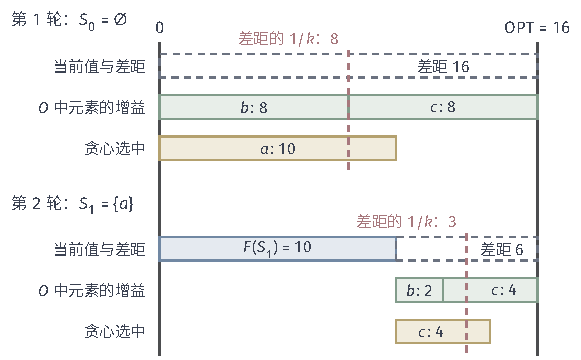
\includegraphics[width=98.446mm]{figures/01-basic-mathematics/04-graphs/tikz/c4-greedy-gap-closing/figure.pdf}
  \caption{贪心每轮至少补上差距的$1/k$（传感器实例，$k=2$，最优集合$O=\{b,c\}$）。每轮上行是当前值（蓝色）与到最优值$16$的差距（虚线框）；中行是$O$中元素相对于当前集合的增益（绿色），它们首尾相接至少覆盖整个差距；红色虚线标出差距的$1/k$，$O$中至少有一个元素的增益越过它；下行是贪心选中元素的增益（黄色），它不小于$O$中任何元素的增益。}
  \label{fig:graph-setfn-greedy-gap-closing}
\end{figure}

一般情形的论证与此相同。最优集合至多有$k$个元素，它们合起来能补上全部差距；由次模性，每个元素相对于当前集合的增益不小于它在“合起来补”时的那一份，所以这些增益之和不少于差距，其中最大者至少是差距的$1/k$。

贪心每轮至少补上剩余差距的$1/k$，差距每轮至多保留原来的$1-1/k$，经过$k$轮至多剩下$(1-1/k)^k$，不超过$e^{-1}$。这就像每期至少偿还剩余欠款的$1/k$，欠款按几何级数下降。

\begin{theorem}[贪心的近似保证]
\label{thm:graph-setfn-greedy-guarantee}
设$F$是有限底集$V$上的集合函数，满足$F(\varnothing)=0$、单调非减且次模；整数$1\leq k\leq|V|$。记$\mathrm{OPT}$为问题~\eqref{eq:graph-setfn-cardinality-problem}的最优值，$S_\ell$为算法~\ref{alg:graph-setfn-greedy}执行$\ell$轮后的集合（$0\leq\ell\leq k$）。则
\begin{equation}
  F(S_\ell)\geq\Bigl(1-\bigl(1-\tfrac1k\bigr)^{\ell}\Bigr)\mathrm{OPT}.
  \label{eq:graph-setfn-greedy-bound}
\end{equation}
特别地，
\[
  F(S_k)\geq\bigl(1-(1-1/k)^k\bigr)\mathrm{OPT}\geq(1-e^{-1})\mathrm{OPT}.
\]
\end{theorem}

\begin{proof}
固定一个最优集合$O$，$|O|\leq k$，$F(O)=\mathrm{OPT}$。考察第$t$轮开始时的集合$S_{t-1}$（$1\leq t\leq k$），先用次模性把它与最优值的差距上界为若干个边际增益之和。把$O\setminus S_{t-1}$中的元素排成$o_1,\ldots,o_r$，由单调性和式~\eqref{eq:graph-setfn-telescoping}，
\[
  \begin{aligned}
  \mathrm{OPT}=F(O)&\leq F(O\cup S_{t-1})\\
  &=F(S_{t-1})+\sum_{j=1}^{r}\Delta\bigl(o_j\mid S_{t-1}\cup\{o_1,\ldots,o_{j-1}\}\bigr).
  \end{aligned}
\]
每个$o_j$都不在$S_{t-1}\cup\{o_1,\ldots,o_{j-1}\}$中，由式~\eqref{eq:graph-setfn-diminishing-returns}，第$j$项满足
\[
  \Delta\bigl(o_j\mid S_{t-1}\cup\{o_1,\ldots,o_{j-1}\}\bigr)\leq\Delta(o_j\mid S_{t-1}).
\]
而贪心在第$t$轮选的是增益最大的元素，所以
\[
  \Delta(o_j\mid S_{t-1})\leq\Delta(v_t\mid S_{t-1})=F(S_t)-F(S_{t-1}).
\]
又$r\leq|O|\leq k$，且每一项增益非负，于是
\[
  \mathrm{OPT}-F(S_{t-1})\leq k\bigl(F(S_t)-F(S_{t-1})\bigr).
\]
也就是说，最优集合的至多$k$个元素合起来能补上的差距，至少有$1/k$能被当前最好的单个元素补上。

记差距$\delta_t=\mathrm{OPT}-F(S_t)$。上式可写成
\[
  \delta_{t-1}\leq k(\delta_{t-1}-\delta_t),
\]
即
\[
  \delta_t\leq\Bigl(1-\frac1k\Bigr)\delta_{t-1},\qquad t=1,\ldots,k.
\]
由$F(\varnothing)=0$得$\delta_0=\mathrm{OPT}$，连续使用$\ell$次得
\[
  \delta_\ell\leq(1-1/k)^\ell\,\mathrm{OPT},
\]
移项即为所求。

最后比较$(1-1/k)^k$与$e^{-1}$。函数$\psi(x)=e^{-x}-(1-x)$满足$\psi(0)=0$，导数$\psi'(x)=1-e^{-x}$在$x>0$时为正，所以$\psi$在$[0,+\infty)$上单调递增：闭区间上连续、内部导数为正的函数严格递增，这是微分中值定理的推论（可参考\BookChapterRef{chap:univariate-differentiation}{卷一“一元函数的微分”章}）。从而
\[
  0\leq1-x\leq e^{-x},\qquad 0\leq x\leq1.
\]
取$x=1/k$再求$k$次幂，得到
\[
  (1-1/k)^k\leq e^{-1}.
\]
\end{proof}

证明中三个条件各有作用。归一化保证差距从$\mathrm{OPT}$开始；若$F(\varnothing)\neq0$，给$F$加上一个常数会改变$F(S_k)$与$\mathrm{OPT}$的比值，比例式就失去意义。单调性用在$F(O)\leq F(O\cup S_{t-1})$和增益非负两处，次模性用在把$O$中元素的增益统一换成相对于$S_{t-1}$的增益。

$k=1$时界为$1$，贪心选出的就是最好的单元素；$k=2$时界为$3/4$。在传感器实例中逐轮核对定理给出的下界：
\[
  \begin{aligned}
  \ell=1:&\quad \tfrac12\times16=8\leq F(S_1)=10,\\
  \ell=2:&\quad \tfrac34\times16=12\leq F(S_2)=14,
  \end{aligned}
\]
两轮都与定理一致。

$1-e^{-1}\approx0.632$是对一切$k$都成立的比例，但它只是近似保证，贪心并不保证精确最优。

\paragraph{复杂度}
第$t$轮要对$n-t+1$个未选元素各求值一次，总共
\[
  \sum_{t=1}^{k}(n-t+1)\leq nk
\]
次求值，再加上开始时的一次$F(\varnothing)$。传感器实例$n=4$、$k=2$，共$1+4+3=8$次。若一次求值的代价为$\tau$（例如覆盖量需要合并若干覆盖范围），总代价是$O(nk\tau)$，选最大值等其余操作只占$O(nk)$。与枚举相比，$nk$次求值随$n,k$多项式增长，而可行子集的个数随$k$迅速增长。

\paragraph{适用范围}
撤去次模性，保证就不再成立。图~\ref{fig:graph-setfn-property-counterexamples}(a)的函数
\[
  F(S)=\max\bigl\{3\,\mathbb I\{\{1,2\}\subseteq S\},\ \mathbb I\{3\in S\}\bigr\}
\]
单调、归一化，但不是次模的。取$k=2$：第$1$轮三个增益依次为$0,0,1$，选$3$；第$2$轮相对于$\{3\}$，加入$1$或$2$的增益都是$0$，按编号选$1$，得到$F(\{1,3\})=1$。最优集合是$\{1,2\}$，$\mathrm{OPT}=3$。

元素$1,2$只有同时选中才有价值，每一轮单独看它们的增益都是零，贪心永远看不到这个互补组合。对照上面的差距论证，这里$O=\{1,2\}$合起来能补上差距$3$，各自的增益却都是$0$，“各元素增益之和不少于差距”这一步失效。把$3$换成任意大的$M$，比例$1/M$可以任意小，所以没有次模性就没有固定比例的保证。

撤去单调性同样会造成损失。图~\ref{fig:graph-setfn-property-counterexamples}(b)的单边割权是次模的，但不单调。取$k=2$并按算法~\ref{alg:graph-setfn-greedy}强制选满：第$1$轮选$1$（增益$1$），第$2$轮只剩$2$，增益为$-1$，仍须加入，结果$\operatorname{cut}(\{1,2\})=0$，而至多选两个时的最优值是$1$。在增益为负时停止可以避免这个例子中的损失，但对一般的非单调次模函数，这样修改后的贪心仍没有定理~\ref{thm:graph-setfn-greedy-guarantee}那样的保证，需要另外的算法与分析，本节不展开。

所以定理~\ref{thm:graph-setfn-greedy-guarantee}只适用于在基数约束下最大化归一化、单调、次模的集合函数，在这一范围内，贪心用至多$nk+1$次求值换来比例保证。贪心规则本身对任何集合函数都能执行，但目标、约束或函数性质改变时，保证都需要重新论证；下一节的预算约束就是一例。

\subsection{惰性贪心}
\label{sec:graph-setfn-lazy-greedy}

\subsubsection{问题与思路}

普通贪心每轮都重算全部未选元素的增益，其中许多元素的旧增益已经远低于领先者，本轮不可能被选中。次模性提供了一个省力的办法：已选集合只会变大，由式~\eqref{eq:graph-setfn-diminishing-returns}，元素的增益只会变小，所以早先算出的增益是它当前增益的上界。若某个元素刚刚重算出的增益不小于其他所有元素的旧增益，它就不小于这些元素的当前增益，可以直接选中，其余元素不必重算。

在实例的第$2$轮，三个候选的旧增益是$b{:}8$、$c{:}8$、$d{:}1$。先重算$b$，得$2$，它不再领先；再重算$c$，得$4$，不小于$b$的新值$2$与$d$的旧值$1$。$d$的当前增益不会超过$1$，不必重算，选$c$。这一轮只做了$2$次求值，选择与普通贪心相同。按这种方式缓存旧增益、只在必要时重算的实现称为\term{惰性贪心}（lazy greedy）。

\subsubsection{算法实现}

\paragraph{缓存增益的优先队列}
每轮都要找出缓存增益最大的元素，并在某个元素的增益重算后把它放回合适的位置，这由以缓存增益为键的最大优先队列完成。每个未选元素$v$在队列中恰有一个条目$(v,g_v,r_v)$：$g_v$是缓存的增益，$r_v$是算出它的轮次，即$g_v=\Delta(v\mid S_{r_v-1})$。轮次$r_v$用来判断缓存是否过期：$r_v$等于当前轮次时，$g_v$就是相对于当前集合的增益。

键的次序按$g_v$从大到小，$g_v$相同时编号小者在前，与普通贪心的平局规则一致。用到的操作只有两个：取出最前的条目，以及插入一个条目。用二叉堆实现时，两者都需要$O(\log n)$次比较。

\paragraph{惰性贪心的实现}
与算法~\ref{alg:graph-setfn-greedy}相同，底集、$k$和求值规则在运行前给定；此外要求$F$是次模的，否则旧增益不是上界，下面的选择可能与普通贪心不同。算法维护四项状态：
\begin{itemize}
  \item 已选集合$S$：初值为空集；
  \item 当前值$F(S)$：初值为一次求值得到的$F(\varnothing)$；
  \item 当前轮次$t$：正在进行的轮次，初值为$1$；
  \item 优先队列：每个未选元素一个条目$(v,g_v,r_v)$，初值$g_v=\Delta(v\mid\varnothing)$、$r_v=1$，由$n$次求值得到。
\end{itemize}
初始化共需$1+n$次求值，第$1$轮的缓存因此全部是新的。每一步取出队列最前的条目$(u,g_u,r_u)$，按两种情形处理：
\begin{itemize}
  \item 若$r_u=t$，缓存是新的：选中$u$，令$S\gets S\cup\{u\}$，$F(S)\gets F(S)+g_u$，$t\gets t+1$；
  \item 若$r_u<t$，缓存已过期：求值一次，令$g_u\gets\Delta(u\mid S)$、$r_u\gets t$，把条目放回队列。
\end{itemize}
$|S|=k$时停止，输出$S$。

\begin{algorithm}[惰性贪心]
\label{alg:graph-setfn-lazy-greedy}
输入：有限底集$V$（元素已编号），整数$0\leq k\leq|V|$，单调非减且次模的集合函数$F$的求值规则。输出：与算法~\ref{alg:graph-setfn-greedy}相同的集合。
\begin{enumerate}
  \item 令$S=\varnothing$，记录$F(\varnothing)$，$t=1$；对每个$v\in V$求$g_v=\Delta(v\mid\varnothing)$，令$r_v=1$，把$(v,g_v,r_v)$插入队列。
  \item 当$|S|<k$时，取出队列最前的条目$(u,g_u,r_u)$。
  \item 若$r_u=t$，令$S\gets S\cup\{u\}$，$F(S)\gets F(S)+g_u$，$t\gets t+1$；否则求$g_u=\Delta(u\mid S)$，令$r_u=t$，把条目放回队列。回到第2步。
  \item 输出$S$。
\end{enumerate}
\end{algorithm}

\paragraph{执行过程}
为了看到旧缓存跨越两轮的情形，在传感器实例上取$k=3$。初始化求值$F(\varnothing)=0$与四个单元素增益，队列为$a{:}10$、$b{:}8$、$c{:}8$、$d{:}1$，轮次都是$1$。表~\ref{tab:graph-setfn-lazy-trace}逐步列出取出的条目、所做的处理和处理后的队列。
\begin{itemize}
  \item 第$1$轮：取出$a$，缓存是新的，直接选中，$S=\{a\}$，$F=10$。
  \item 第$2$轮：取出$b$，缓存来自第$1$轮，重算得$2$后放回；取出$c$，重算得$4$后放回，排到最前；再取出$c$，缓存是新的，选中，$S=\{a,c\}$，$F=14$。$d$的旧值$1$始终排在后面，没有重算。
  \item 第$3$轮：取出$b$，它的缓存$2$来自第$2$轮，已过期，重算仍得$2$后放回；再取出$b$，选中，$S=\{a,b,c\}$，$F=16$。
\end{itemize}
此时$|S|=3$，停止。三轮的选择与普通贪心逐轮重算的结果一致，求值共$1+4+2+1=8$次，普通贪心需要$1+4+3+2=10$次。

\begin{table}[!htb]
  \centering
  \caption{传感器实例上$k=3$的惰性贪心。每行是一次取出：“重算”表示缓存过期而求值一次后放回，“选中”表示缓存是新的；队列按键的次序列出，每项写元素、缓存增益与算出它的轮次。}
  \label{tab:graph-setfn-lazy-trace}
  \small
  \begin{tabular}{@{}cccl@{}}
    \toprule
    轮 & 取出 & 处理 & 处理后的队列 \\
    \midrule
    初始 & — & 求值$5$次 & $a(10,1)$，$b(8,1)$，$c(8,1)$，$d(1,1)$ \\
    $1$ & $a(10,1)$ & 选中 & $b(8,1)$，$c(8,1)$，$d(1,1)$ \\
    $2$ & $b(8,1)$ & 重算得$2$ & $c(8,1)$，$b(2,2)$，$d(1,1)$ \\
    $2$ & $c(8,1)$ & 重算得$4$ & $c(4,2)$，$b(2,2)$，$d(1,1)$ \\
    $2$ & $c(4,2)$ & 选中 & $b(2,2)$，$d(1,1)$ \\
    $3$ & $b(2,2)$ & 重算得$2$ & $b(2,3)$，$d(1,1)$ \\
    $3$ & $b(2,3)$ & 选中 & $d(1,1)$ \\
    \bottomrule
  \end{tabular}
\end{table}

\subsubsection{算法分析}

\paragraph{正确性}
惰性贪心每轮选出的元素与普通贪心按同一平局规则选出的相同，从而定理~\ref{thm:graph-setfn-greedy-guarantee}的保证原样适用。证明对轮次归纳：设前$t-1$轮两者选出相同元素，当前集合都是$S_{t-1}$。

在第$t$轮，设取出的条目$(u,g_u,t)$缓存是新的，则$g_u=\Delta(u\mid S_{t-1})$。对队列中任一其他元素$v$，它的缓存$g_v=\Delta(v\mid S_{r_v-1})$是在更小的集合$S_{r_v-1}\subseteq S_{t-1}$上算出的，由式~\eqref{eq:graph-setfn-diminishing-returns}，
\[
  g_v\geq\Delta(v\mid S_{t-1}).
\]
$u$排在$v$前面，所以
\[
  \Delta(u\mid S_{t-1})=g_u\geq g_v\geq\Delta(v\mid S_{t-1}).
\]
若某个$v$的当前增益与$u$相等，则$g_v$也与$g_u$相等，$u$排在前面说明它的编号更小。所以$u$正是普通贪心第$t$轮的选择。

每一轮都会结束：每次重算都把一个过期条目变成新的，一轮内至多重算$n-t+1$次，之后队列最前的条目必定是新的而被选中。

这里的正确性只用到次模性，没有用到单调性和归一化；它们是近似保证需要的条件。对一般函数，旧增益不是上界，排在后面的元素的当前增益可能已经超过选中的元素，因此必须每轮全部重算。

\paragraph{复杂度}
初始化需要$1+n$次求值。第$t\geq2$轮的重算次数不超过未选元素个数$n-t+1$，所以最坏情形的求值次数与普通贪心相同；省下多少取决于增益下降的快慢，没有一般的保证。

每次重算伴随一次取出与一次插入，每轮再有一次取出用于选中，每次队列操作需要$O(\log n)$次比较，最坏总开销为$O(nk\log n)$次比较，另加初始插入的$O(n\log n)$次比较。队列存放$n$个条目，额外空间为$O(n)$。一次求值的代价$\tau$通常远大于$O(\log n)$，这时省下的求值次数决定了实际运行时间。

% 第9章第2节：预算约束下的子集选择（问题与思路；算法实现；算法分析）。

\section{预算约束下的子集选择}
\label{sec:graph-budget-selection}

基数约束让每个元素占用一个名额。实际中不同传感器的价格不同，限制的往往是总花费而不是个数。逐轮贪心仍然可用，但比较的对象要改成单位成本的增益。本节说明这一改动的理由与实现，再用反例说明上一节的近似保证不能直接搬到预算约束下。

\subsection{问题与思路}
\label{sec:graph-setfn-budget-problem}

给每个元素$v\in V$指定成本$c_v$，再给定总预算$B\geq0$。要求的是
\begin{equation}
  \max_{S\subseteq V}\ F(S)\qquad\text{满足}\quad\sum_{v\in S}c_v\leq B.
  \label{eq:graph-setfn-budget-problem}
\end{equation}
满足成本条件的子集称为预算可行的，这一条件称为\term{预算约束}（budget constraint）。目标函数$F$与上一节相同，改变的只是允许的子集。所有成本都取$1$、预算取$k$时，预算约束就是基数约束，所以本节的问题是上一节的推广。

成本为零的元素需要先单独处理。零成本元素不占预算，若$F$单调，把它们全部加入不会降低目标，可以在开始时一次放进集合；若$F$不单调，它们是否值得加入要看增益的正负。以下设所有成本为正。另外，成本超过$B$的元素不可能出现在任何可行集合中，可以预先删去。

下面在传感器实例上取第~\ref{sec:graph-setfn-definition}小节的成本，并给定预算：
\[
  c_a=4,\quad c_b=3,\quad c_c=4,\quad c_d=1,\qquad B=7.
\]
预算可行的子集共有$10$个：空集、四个单元素集，以及$\{a,b\}$（成本$7$）、$\{a,d\}$（$5$）、$\{b,c\}$（$7$）、$\{b,d\}$（$4$）、$\{c,d\}$（$5$）；三元及以上的子集成本都超过$7$。枚举得最优集合为$\{b,c\}$，覆盖$16$格。

与$k=2$的基数约束相比，$\{a,c\}$成本为$8$，现在不可行了；而$\{a,b\}$在两种约束下都可行。选择的个数不再直接决定资源消耗，每次加入元素前都要检查剩余预算。

把上一节的贪心原样搬过来，就是每轮在付得起的元素里选增益最大的。这样做可能偏爱昂贵的元素：一个元素增益大，可能只是因为它贵，而它占去的预算本可以换来更多增益。预算是按成本消耗的，所以更合理的比较是每单位成本带来多少增益，即比值$\Delta(v\mid S)/c_v$。

这样得到单位成本规则：每轮选比值最大且付得起的元素，直到剩余预算放不下任何元素，或者付得起的元素都不再带来增益。

\subsection{算法实现}
\label{sec:graph-setfn-ratio-greedy}

成本$c_v$、预算$B$和求值规则在运行前给定，运行中不变，不算状态。与上一节相比，算法多记录剩余预算，并且每轮只在付得起的元素中比较。算法维护四项状态：
\begin{itemize}
  \item 已选集合$S$：初值为空集；
  \item 剩余预算$R=B-\sum_{v\in S}c_v$：初值为$B$；
  \item 当前值$F(S)$：初值由一次求值得到$F(\varnothing)$，此后每轮加上选中元素的增益；
  \item 本轮增益：每个付得起的未选元素$v$相对于当前$S$的增益$\Delta(v\mid S)$，每轮重新计算。
\end{itemize}
初始化令$S=\varnothing$、$R=B$，并求值一次得到$F(\varnothing)$。每一轮做四件事：
\begin{itemize}
  \item 列候选：记$Q=\{v\in V\setminus S:c_v\leq R\}$为付得起的未选元素；若$Q$为空，停止；
  \item 求增益：对每个$v\in Q$求值，得到$\Delta(v\mid S)$；若这些增益全为零，停止；
  \item 选择：取比值$\Delta(v\mid S)/c_v$最大的$v$，比值相同时取编号最小者；
  \item 更新：令$F(S)\gets F(S)+\Delta(v\mid S)$，再令$S\gets S\cup\{v\}$，$R\gets R-c_v$。
\end{itemize}
停止条件因此有两个：剩余预算放不下任何未选元素，或者付得起的元素都不再增加目标。

\begin{algorithm}[预算约束下的单位成本贪心]
\label{alg:graph-setfn-ratio-greedy}
输入：有限底集$V$（元素已编号），正成本$c_v$，预算$B\geq0$，单调非减集合函数$F$的求值规则。输出：预算可行的集合。
\begin{enumerate}
  \item 令$S=\varnothing$，$R=B$，记录$F(\varnothing)$。
  \item 记候选集合$Q=\{v\in V\setminus S:c_v\leq R\}$。若$Q$为空，停止。
  \item 对每个$v\in Q$计算$\Delta(v\mid S)$。若这些增益全为零，停止；否则取比值$\Delta(v\mid S)/c_v$最大的$v$，比值相同时取编号最小者。
  \item 令$S\leftarrow S\cup\{v\}$，$R\leftarrow R-c_v$，回到第2步。
\end{enumerate}
\end{algorithm}

\paragraph{执行过程}
在$B=7$的实例上，表~\ref{tab:graph-setfn-ratio-trace}逐轮记录状态。
\begin{itemize}
  \item 第$1$轮：$R=7$，四个元素都付得起，增益是各自的覆盖量，比值依次为
  \[
    a{:}\ 10/4=2.5,\quad b{:}\ 8/3\approx2.67,\quad c{:}\ 8/4=2,\quad d{:}\ 1/1=1.
  \]
  选$b$，$R=4$。
  \item 第$2$轮：$Q=\{a,c,d\}$，增益相对于$\{b\}$重新计算。$a$只补上第$5$、$6$列的$4$格，比值$1$；$c$与$b$不重叠，增益$8$，比值$2$；$d$那一格已被$b$覆盖，增益$0$。选$c$，$R=0$。
  \item 第$3$轮：没有成本不超过$0$的元素，$Q$为空，停止。
\end{itemize}
输出$\{b,c\}$，覆盖$16$格，恰为枚举最优值。

\begin{table}[!htb]
  \centering
  \caption{$B=7$时单位成本贪心的状态表（成本$c_a=4$、$c_b=3$、$c_c=4$、$c_d=1$）。每格写增益，括号内为增益与成本之比；“—”表示已选或付不起；最后一列是本轮选中的元素与更新后的剩余预算。}
  \label{tab:graph-setfn-ratio-trace}
  \small
  \begin{tabular}{@{}cccccccc@{}}
    \toprule
    轮 & $S$ & $R$ & $a$ & $b$ & $c$ & $d$ & 选中，新$R$ \\
    \midrule
    $1$ & $\varnothing$ & $7$ & $10\ (2.5)$ & $8\ (2.67)$ & $8\ (2)$ & $1\ (1)$ & $b$，$4$ \\
    $2$ & $\{b\}$ & $4$ & $4\ (1)$ & — & $8\ (2)$ & $0\ (0)$ & $c$，$0$ \\
    $3$ & $\{b,c\}$ & $0$ & — & — & — & — & $Q$为空，停止 \\
    \bottomrule
  \end{tabular}
\end{table}

作为对照，按总增益最大选择的规则在第$1$轮选$a$（增益$10$），剩余预算$3$；第$2$轮付得起的有$b$（增益$2$）和$d$（增益$1$），$c$的成本$4$超出剩余预算，选$b$，剩余预算$0$，停止，覆盖$12$格。图~\ref{fig:graph-setfn-budget-rule-comparison}把两种规则的选择画在同一条预算上：昂贵的$a$一开始就占去一半以上的预算，之后只剩小元素可选。

\begin{figure}[!htb]
  \centering
  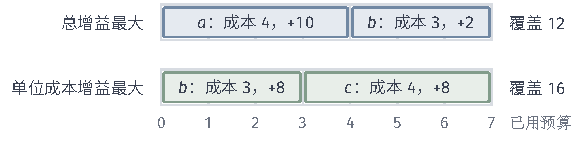
\includegraphics[width=98.538mm]{figures/01-basic-mathematics/04-graphs/tikz/c4-budget-rule-comparison/figure.pdf}
  \caption{预算$B=7$下两种逐轮规则的选择结果（成本$c_a=4$、$c_b=3$、$c_c=4$、$c_d=1$）。每条横条代表$7$个单位的预算，色块的宽度是所选元素的成本，块内写出选择时的增益。按总增益先选昂贵的$a$，剩余预算只够再选增益$2$的$b$，覆盖$12$格；按单位成本先选$b$，再选$c$，覆盖$16$格。}
  \label{fig:graph-setfn-budget-rule-comparison}
\end{figure}

\paragraph{最佳单元素比较}
单位成本规则也有自己的偏差：它可能先选几个便宜的小元素，把预算切碎，使一个昂贵但价值很高的元素再也放不进去。

一种简单的补救是在算法结束后增加一步：计算每个可行单元素的值$F(\{v\})$（$c_v\leq B$），输出$S$与最佳单元素中函数值较大的一个。这只需另外$n$次求值。

在$B=7$的实例中，最佳单元素是$\{a\}$，覆盖$10$格，小于$16$，输出仍是$\{b,c\}$。这一检查只是一个具体策略；本节没有给出它的分析，因此不附加任何近似比例。

\subsection{算法分析}
\label{sec:graph-setfn-budget-limits}

\paragraph{可行性}
算法始终保持$R=B-\sum_{v\in S}c_v\geq0$：初始时$R=B\geq0$；每轮只从$Q$中选元素，而$Q$中元素的成本不超过$R$，减去后$R$仍非负。所以输出总是预算可行的。

\paragraph{停止性}
每轮加入一个新元素，至多执行$n$轮就会停止。停止时有两种原因：没有付得起的元素，或者付得起的元素都不再增加目标。

对单调函数，后一种情形下再加入任何一个付得起的元素都不会提高函数值；若函数还是次模的，按上一节提前停止的论证，一次加入若干个付得起的元素也不会提高函数值。

\paragraph{复杂度}
第$t$轮的候选元素不超过$n-t+1$个，所以求值次数不超过
\[
  n+(n-1)+\cdots+1=\frac{n(n+1)}{2},
\]
再加开始时的一次$F(\varnothing)$；附加最佳单元素比较时另加$n$次。上面的实例做了$1+4+3=8$次求值。若一次求值的代价为$\tau$，总代价为$O(n^2\tau)$。

\paragraph{适用范围}
单位成本规则在上面的实例中表现很好，但它本身没有任何固定比例的保证。

\begin{example}[比值规则的失效]
\label{ex:graph-setfn-ratio-failure}
底集$\{u,w\}$，预算$B=100$。$u$的成本为$1$、价值为$2$，$w$的成本为$100$、价值为$100$，目标取模函数$F(S)=\sum_{v\in S}(\text{价值})$。各价值非负，所以它归一化、单调，也是次模的。

比值规则第$1$轮比较$2/1=2$与$100/100=1$，选$u$；剩余预算$99<100$，$w$付不起，算法停止，得$F(\{u\})=2$。最优选择是$\{w\}$，$F=100$。见图~\ref{fig:graph-setfn-budget-ratio-failure}。

把$w$的成本、价值与预算同时换成任意大的$M$，比值规则仍先选$u$，得到$2$而最优值为$M$，比例$2/M$可以任意小。
\end{example}

\begin{figure}[!htb]
  \centering
  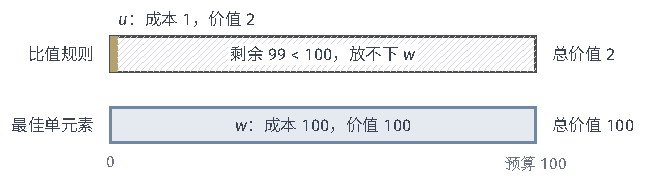
\includegraphics[width=109.146mm]{figures/01-basic-mathematics/04-graphs/tikz/c4-budget-ratio-failure/figure.pdf}
  \caption{比值规则的失效例。横条长度代表预算$100$。上行：比值规则先选单位价值较高的$u$（黄色，成本$1$，为便于观察略加宽），剩余$99$个单位（斜线）放不下成本$100$的$w$，总价值$2$。下行：最佳单元素$w$恰好用满预算，总价值$100$。}
  \label{fig:graph-setfn-budget-ratio-failure}
\end{figure}

这个例子的目标是模函数，从而归一化、单调且次模，满足上一节定理的全部函数条件。比值规则仍不能继承那里的保证，原因在于上一节差距论证的关键一步没有对应物。

那里最优集合的至多$k$个元素在每一轮都仍然可选，所以当前最好的元素至少补上差距的$1/k$。预算约束下，选进一个便宜元素就可能让最优集合中的元素再也付不起：例中选了$u$以后，差距是$100-2=98$，而最优集合唯一的元素$w$已经放不进剩余的$99$个单位，可选的元素一个也没有，差距一点也补不上。

最佳单元素比较能修复这个例子，但修复一个例子不构成一般保证；有严格保证的预算选择算法需要另外的枚举或修正机制及其证明，本书不展开。

\paragraph{结果检验}
小实例可以枚举全部预算可行子集，核对总成本、函数值以及与最优值的差距：$B=7$时比值规则的$\{b,c\}$与枚举最优一致，总增益规则的$\{a,b\}$差$4$格。

大实例无法枚举时，至少应报告剩余预算、最终目标值、最佳单元素的值和总求值次数；若逐轮规则的结果不如最佳单元素，往往就是出现了示例~\ref{ex:graph-setfn-ratio-failure}那样预算被小元素切碎的情形。

\paragraph{与基数约束贪心的比较}
两种贪心的状态与更新几乎相同，差别只在选择依据换成单位成本的增益，停止条件换成剩余预算放不下有增益的元素。所有成本都取$1$、预算取$k$时，单位成本规则除了增益全为零时提前停止以外，就是上一节的贪心。

对同样的归一化单调次模目标，基数约束下有$1-(1-1/k)^k$的保证，预算约束下简单的比值规则却可以任意差：约束的形式本身就决定算法能否得到保证。

\FloatBarrier
\section{本章小结}
\label{sec:subset-selection-chapter-summary}

本章回答了名额或经费有限时怎样选子集。两种贪心有相同的骨架：从空集出发，逐轮维护已选集合与当前值，相对于当前集合重算增益，加入一个元素。基数约束下比较的是边际增益本身，预算约束下比较的是单位成本的增益，并且只在付得起的元素中比较。两者都只需多项式次求值，分别至多$nk+1$次和$n(n+1)/2+1$次，总代价还要乘以每次求值的开销。

贪心规则本身对任何集合函数都能执行，但结果有没有保证取决于目标性质和约束。基数约束下最大化归一化、单调、次模的函数时，最优集合的至多$k$个元素在每一轮都仍然可选；由次模性，当前最好的元素至少补上剩余差距的$1/k$，差距按几何级数缩小，贪心值不低于最优值的$1-(1-1/k)^k$倍，从而不低于$1-e^{-1}$倍。撤去次模性，贪心看不到只有同时选中才有价值的互补组合；撤去单调性，强制选满会降低目标。两种情形下比例保证都不再成立。

惰性贪心是同一规则的另一种实现。次模性使旧增益成为当前增益的上界，优先队列据此只重算排在最前的元素；在一致的平局规则下，它与普通贪心逐轮选出相同的元素，所以继承同样的保证。它的正确性只需要次模性，节省多少求值没有一般的保证，最坏情形与普通贪心相同。

预算约束改变了可行性，也改变了分析。单位成本规则在传感器实例中找到最优解，却在成本与价值分别为$(1,2)$与$(100,100)$的例子中可以任意差：选进便宜元素以后，最优集合的元素可能再也放不进剩余预算，差距论证中“最优集合的元素仍可选”这一步失效。最佳单元素比较能修复这个例子，但本章没有证明它的一般比例。使用任何一种选择方法之前，都要写明目标方向、约束形式、函数是否归一化、单调和次模。

下一章转向最小化方向，没有基数或预算约束，但要求目标由一元项和成对项组成；在相应的次模条件下，最小割给出精确解。


% 第10章：成对二值函数的最小化（问题与思路；次模条件与割表示；算法实现；算法分析；本章小结）。

\chapter{成对二值函数的最小化}
\label{sec:graph-pairwise-binary-cut}
\label{chap:pairwise-binary-minimization}

给一张图的每个顶点贴上“前景”或“背景”两种标签：每个顶点各自有偏好，相邻顶点又希望标签一致，代价写成每个顶点的成本加上每条边的成本。这样的目标是一个二值配置的函数，$n$个顶点有$2^n$种配置，逐一枚举很快不可行。本章要回答：这类只由一元项和成对项组成的二值目标，什么时候可以不枚举而精确求出最小值，怎样求，以及结果怎样核对。

上一章在约束下最大化集合函数，贪心只给出有比例保证的近似解，保证依赖单调、次模和约束形式。本章换一个方向：目标是最小化，没有基数或预算约束，但函数必须具有一元加成对的结构。第~\ref{sec:graph-setfn-pairwise-problem}节给出问题，并说明逐点选择为什么不够。第~\ref{sec:graph-setfn-cut-representation}节说明割容量能表示哪些成本，导出成对项的次模条件，并证明条件成立时每个配置的成本等于一个常数加上对应割的容量。

后两节把这一表示变成算法并加以检验。第~\ref{sec:graph-setfn-cut-solving}节逐项合并一元成本、移出常数、构造非负容量网络，调用第~\ref{chap:max-flow-min-cut}章的最大流算法，再由割的两侧读出配置。第~\ref{sec:graph-setfn-cut-analysis}节用割表示与最大流最小割定理证明结果全局最优，给出复杂度和独立核对的办法，并说明非次模成对项、高阶项和附加约束为什么不能直接处理。本章用到第~\ref{chap:set-functions}章的指示向量与次模不等式，以及第~\ref{chap:max-flow-min-cut}章的$s$--$t$割、最大流最小割定理和Edmonds--Karp算法。

\section{问题与思路}
\label{sec:graph-setfn-pairwise-problem}

给底集$V$的每个元素$i$一个二值变量$x_i\in\{0,1\}$，$x_i=1$表示选中$i$，于是配置$\bm x\in\{0,1\}^V$就是第~\ref{sec:graph-setfn-binary-vectors}小节的指示向量。元素之间的交互用无向图$\mathcal G=(V,E)$记录：只有$\{i,j\}\in E$的两个元素之间有成对项。这张\emph{交互图}只记录哪些变量共同出现在成本项中；底集不必来自某张事先给定的图，交互图由目标的写法决定。目标是
\begin{equation}
  \min_{\bm x\in\{0,1\}^V}J(\bm x),\qquad
  J(\bm x)=\sum_{i\in V}\phi_i(x_i)+\sum_{\{i,j\}\in E}\phi_{i,j}(x_i,x_j).
  \label{eq:graph-setfn-pairwise-objective}
\end{equation}
\term{一元项}$\phi_i$给出元素$i$两种状态各自的成本，只有两个数$\phi_i(0),\phi_i(1)$；\term{成对项}$\phi_{i,j}$给出$i,j$四种联合状态的成本，例如两者取值不同时的不一致代价，或两者同时选中的配合收益（以负成本表示）。为了让$\phi_{i,j}(a,b)$的含义确定，对每条边固定一个次序，约定$a$是$x_i$、$b$是$x_j$的值。

本章只考虑有限实值成本。输入是这些成本表，输出是一个使$J$最小的配置$\hat{\bm x}$及其目标值。

通过$S=\{i:x_i=1\}$，$J$也是$V$上的集合函数。但并不是每个集合函数都能写成式~\eqref{eq:graph-setfn-pairwise-objective}的形式：例如只在三个元素同时选中时才产生的成本，不能拆成两两之间的成对项。本章的方法只适用于已经具有这种一元加成对结构的目标。

成对项会改变各元素的最优取值。下面用一个两变量的例子说明，一元项为
\[
  \phi_1(0)=0,\quad \phi_1(1)=1,\qquad \phi_2(0)=2,\quad \phi_2(1)=0,
\]
成对项为
\[
  \begin{gathered}
  \phi_{1,2}(0,0)=0,\qquad \phi_{1,2}(0,1)=3,\\
  \phi_{1,2}(1,0)=5,\qquad \phi_{1,2}(1,1)=0.
  \end{gathered}
\]
图~\ref{fig:graph-setfn-pairwise-config-table}列出四种配置的成本。

若只看一元项，元素$1$偏好$0$，元素$2$偏好$1$，逐点选择得到$(0,1)$，成本为
\[
  J(0,1)=0+0+3=3.
\]
但成对项惩罚两者取值不同，整体最优是$(1,1)$，成本为
\[
  J(1,1)=1+0+0=1.
\]
让元素$1$放弃自己的偏好只多付$1$，却省下了$3$的不一致代价。

\begin{figure}[!htb]
  \centering
  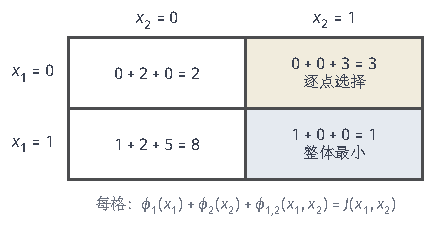
\includegraphics[width=72.383mm]{figures/01-basic-mathematics/04-graphs/tikz/c4-pairwise-config-table/figure.pdf}
  \caption{两变量成对二值函数的四种配置。行是$x_1$，列是$x_2$，每格依次写出$\phi_1(x_1)$、$\phi_2(x_2)$、$\phi_{1,2}(x_1,x_2)$与总成本$J$。逐点按一元项选择得到黄色格$(0,1)$，成本$3$；整体最小是蓝色格$(1,1)$，成本$1$。}
  \label{fig:graph-setfn-pairwise-config-table}
\end{figure}

两个变量可以枚举，$n$个变量则有$2^n$种配置。避开枚举的办法是借助割：在顶点为$V\cup\{s,t\}$的网络中，一个$s$--$t$割由$V$中哪些元素与$s$同侧决定；规定源侧取$0$、汇侧取$1$，割就成了配置。

如果能选非负的弧容量，使每个配置的割容量都等于$J(\bm x)$减去同一个常数，最小割对应的配置就是$J$的最小点，$2^n$种配置的枚举变成一次最大流计算。困难在于割容量只能累加非负容量，而成本可以为负，成对项的四个值也未必能用弧表示。

\section{次模条件与割表示}
\label{sec:graph-setfn-cut-representation}

割容量只累加从源侧指向汇侧的弧。按“源侧取$0$、汇侧取$1$”的约定，每条弧都像一笔只在特定情形下收取的费用。弧$s\to i$在$i$位于汇侧、即$x_i=1$时被割断，相当于对$x_i=1$收费；弧$i\to t$在$x_i=0$时被割断，相当于对$x_i=0$收费；边$\{i,j\}$上方向相反、容量相同的两条弧$i\to j$与$j\to i$，在$x_i\neq x_j$时恰有一条从源侧指向汇侧，相当于对两者取值不同收费。

容量非负，这三类费用也都必须非负。所以要做的是把$J$改写成一个常数加上这三类非负费用；常数与配置无关，不影响哪个配置最小。

一元项只有两个值，减去其中较小者就成为非负的单变量费用，总能改写。困难在成对项。

成对项有四个值，其中三个自由度可以吸收：一个常数，以及只依赖$x_i$或只依赖$x_j$的部分，后两者可以并入一元项。剩下的一个自由度衡量两个变量的相互作用，即两种取值不同的配置比两种取值相同的配置合计多付多少。它只能由“取值不同时收费”的两条弧表示，因而必须非负。

把这一要求写成四个值的关系，就是对每条边$\{i,j\}\in E$成立
\begin{equation}
  \phi_{i,j}(0,0)+\phi_{i,j}(1,1)\leq\phi_{i,j}(0,1)+\phi_{i,j}(1,0).
  \label{eq:graph-setfn-pairwise-submodular}
\end{equation}
它正是两元素底集$\{i,j\}$上的次模不等式：把$\phi_{i,j}$看成$\{i,j\}$上的集合函数，在式~\eqref{eq:graph-setfn-submodular-inequality}中取$X=\{i\}$、$Y=\{j\}$，左边$F(X)+F(Y)$对应$\phi_{i,j}(1,0)+\phi_{i,j}(0,1)$，右边$F(X\cup Y)+F(X\cap Y)$对应$\phi_{i,j}(1,1)+\phi_{i,j}(0,0)$。上面的例子中$0+0\leq3+5$，条件成立。

这个条件也让整个$J$成为次模的。把成对项看成$V$上的集合函数$S\mapsto\phi_{i,j}(\mathbb I\{i\in S\},\mathbb I\{j\in S\})$，它只读取$S\cap\{i,j\}$；加入$i$或$j$以外的元素增益为$0$，加入$i$时的增益只取决于$j$是否已选，式~\eqref{eq:graph-setfn-pairwise-submodular}正是说$j$已选时这个增益不更大，所以它满足边际递减。

一元项之和是模函数。由次模函数之和仍为次模，满足条件时$J$作为集合函数是次模的。

条件成立时，可吸收的三个自由度与相互作用能够显式分开。

\begin{lemma}[成对项的分解]
\label{lem:graph-setfn-pairwise-decomposition}
设$\phi_{i,j}$满足式~\eqref{eq:graph-setfn-pairwise-submodular}，简记$p_{a,b}=\phi_{i,j}(a,b)$，令
\[
  \begin{gathered}
  w_{i,j}=\frac{p_{0,1}+p_{1,0}-p_{0,0}-p_{1,1}}{2},\\
  \alpha_i=p_{1,0}-p_{0,0}-w_{i,j},\qquad
  \alpha_j=p_{0,1}-p_{0,0}-w_{i,j}.
  \end{gathered}
\]
则$w_{i,j}\geq0$，并且对四种配置都有
\begin{equation}
  \phi_{i,j}(x_i,x_j)=p_{0,0}+\alpha_ix_i+\alpha_jx_j+w_{i,j}\,|x_i-x_j|.
  \label{eq:graph-setfn-pairwise-decomposition}
\end{equation}
\end{lemma}

\begin{proof}
$w_{i,j}\geq0$就是式~\eqref{eq:graph-setfn-pairwise-submodular}移项除以$2$。逐个代入四种配置核对右边：
\[
  \begin{aligned}
  (0,0):&\quad p_{0,0},\\
  (1,0):&\quad p_{0,0}+\alpha_i+w_{i,j}=p_{1,0},\\
  (0,1):&\quad p_{0,0}+\alpha_j+w_{i,j}=p_{0,1},\\
  (1,1):&\quad p_{0,0}+\alpha_i+\alpha_j=p_{1,0}+p_{0,1}-p_{0,0}-2w_{i,j}=p_{1,1},
  \end{aligned}
\]
最后一行的末步代入$w_{i,j}$的定义。
\end{proof}

在例子中，按引理算出
\[
  \begin{gathered}
  w_{1,2}=\frac{3+5-0-0}{2}=4,\\
  \alpha_1=5-0-4=1,\qquad \alpha_2=3-0-4=-1.
  \end{gathered}
\]

图~\ref{fig:graph-setfn-pairwise-decomposition}把成对项的$2\times2$成本表拆成四张表之和：常数表全为$0$；$\alpha_1x_1$只随行变化，$\alpha_2x_2$只随列变化，它们稍后并入一元项；剩下的不一致惩罚只在两个非对角格上取$4$，正好由容量为$4$的一对反向弧表示。

\begin{figure}[!htb]
  \centering
  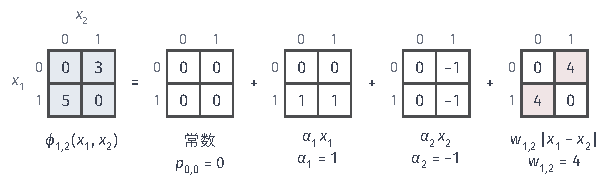
\includegraphics[width=103.103mm]{figures/01-basic-mathematics/04-graphs/tikz/c4-pairwise-decomposition/figure.pdf}
  \caption{两变量例子中成对项的分解（引理~\ref{lem:graph-setfn-pairwise-decomposition}）。每张$2\times2$表的行是$x_1$、列是$x_2$。左边的成本表等于常数$p_{0,0}$、只随$x_1$变化的$\alpha_1x_1$、只随$x_2$变化的$\alpha_2x_2$与不一致惩罚$w_{1,2}|x_1-x_2|$之和，逐格相加可以核对。只有最后一张表（红色格）需要用弧$1\to2$与$2\to1$表示，次模条件保证它的值$w_{1,2}$非负。}
  \label{fig:graph-setfn-pairwise-decomposition}
\end{figure}

\paragraph{一元项的合并与移位}
对每条边作上述分解，把常数$\phi_{i,j}(0,0)$累加起来，把线性部分$\alpha_ix_i$、$\alpha_jx_j$并入相应元素的一元项。记合并后的一元项为$\psi_i$，即$\psi_i(0)=\phi_i(0)$，$\psi_i(1)=\phi_i(1)$加上与$i$关联的各边分解出的$\alpha_i$。注意$\alpha_i$随边而变，同一个$i$在不同的边上分解出的数一般不同，要逐边累加。

$\psi_i$可能取负值，而容量必须非负，所以再令
\[
  m_i=\min\{\psi_i(0),\psi_i(1)\},\qquad \tilde\psi_i=\psi_i-m_i,
\]
两种状态的成本都减去同一个数，$\tilde\psi_i$的两个值非负且至少一个为零。移出的数另行累计成常数
\[
  K=\sum_{\{i,j\}\in E}\phi_{i,j}(0,0)+\sum_{i\in V}m_i .
\]
于是对每个配置都有
\begin{equation}
  J(\bm x)=K+\sum_{i\in V}\tilde\psi_i(x_i)+\sum_{\{i,j\}\in E}w_{i,j}\,|x_i-x_j|,
  \label{eq:graph-setfn-shifted-objective}
\end{equation}
右边除常数$K$外各项都非负。

在例子中，合并一元项得到
\[
  \psi_1=(0,\,1+1)=(0,2),\qquad \psi_2=(2,\,0-1)=(2,-1).
\]
较小值为$m_1=0$、$m_2=-1$，所以移位后
\[
  \tilde\psi_1=(0,2),\qquad \tilde\psi_2=(3,0),
\]
移出的常数为
\[
  K=0+0+(-1)=-1.
\]

\paragraph{网络构造}
由式~\eqref{eq:graph-setfn-shifted-objective}构造有向网络：顶点为$V\cup\{s,t\}$；对每个$i\in V$，建弧$s\to i$，容量$\tilde\psi_i(1)$，以及弧$i\to t$，容量$\tilde\psi_i(0)$；对每条边$\{i,j\}\in E$，建方向相反的两条弧$i\to j$与$j\to i$，容量都是$w_{i,j}$。容量为零的弧可以省略。

配置$\bm x$对应$s$--$t$割$(S_{\bm x},\bar S_{\bm x})$，其中
\[
  S_{\bm x}=\{s\}\cup\{i:x_i=0\};
\]
这是第~\ref{sec:graph-opt-flow-cut}节意义下的$s$--$t$割，割容量只累计从源侧跨向汇侧的弧。用最小割求解这类问题的方法常称为\term{图割}（graph cut）。

\begin{theorem}[成对二值函数的割表示]
\label{thm:graph-setfn-cut-representation}
设式~\eqref{eq:graph-setfn-pairwise-objective}中的成本都是有限实数，且每个成对项满足式~\eqref{eq:graph-setfn-pairwise-submodular}。则在上面构造的网络中，配置与$s$--$t$割一一对应，并且每个配置$\bm x$对应的割容量等于$J(\bm x)-K$。因此最小割对应的配置是$J$的最小点。
\end{theorem}

\begin{proof}
任一$s$--$t$割的源侧都含$s$、不含$t$，由$V$中哪些元素在源侧唯一确定，所以割与配置一一对应。

割容量只累计从源侧指向汇侧的弧，逐类计算。若$x_i=0$，$i$在源侧，弧$i\to t$跨出，计入$\tilde\psi_i(0)$，弧$s\to i$两端都在源侧，不计入；若$x_i=1$，$i$在汇侧，弧$s\to i$跨出，计入$\tilde\psi_i(1)$，弧$i\to t$两端都在汇侧，不计入。两种情形合起来恰好计入$\tilde\psi_i(x_i)$。

对边$\{i,j\}$，若$x_i=x_j$，两条弧都不跨越；若$x_i\neq x_j$，两条反向弧中恰有一条从源侧指向汇侧，计入一次$w_{i,j}$。合起来恰好计入$w_{i,j}|x_i-x_j|$。

所以割容量等于式~\eqref{eq:graph-setfn-shifted-objective}右边去掉$K$，即$J(\bm x)-K$。$K$与配置无关，最小化割容量与最小化$J$是同一件事。
\end{proof}

在例子中，网络有弧$s\to1$（容量$2$）、$2\to t$（容量$3$）、$1\to2$与$2\to1$（容量都是$4$），弧$1\to t$与$s\to2$容量为零。表~\ref{tab:graph-setfn-cut-check}逐个核对四种配置：割容量都比$J$大$1$，即$-K$。

\begin{table}[!htb]
  \centering
  \begin{tabular}{cccc}
    \toprule
    配置$\bm x$ & 源侧 & 跨出的正容量弧 & 割容量 / $J(\bm x)$ \\
    \midrule
    $(0,0)$ & $\{s,1,2\}$ & $2\to t$ & $3$ / $2$ \\
    $(0,1)$ & $\{s,1\}$ & $1\to2$ & $4$ / $3$ \\
    $(1,0)$ & $\{s,2\}$ & $s\to1$，$2\to t$，$2\to1$ & $9$ / $8$ \\
    $(1,1)$ & $\{s\}$ & $s\to1$ & $2$ / $1$ \\
    \bottomrule
  \end{tabular}
  \caption{两变量例子中四种配置的割容量与原目标值。源侧元素取$0$、汇侧元素取$1$；每行割容量都等于$J(\bm x)+1$，相差的常数是$-K=1$，所以割容量最小的$(1,1)$也是$J$的最小点。}
  \label{tab:graph-setfn-cut-check}
\end{table}

\section{算法实现}
\label{sec:graph-setfn-cut-solving}

交互图、一元成本表和成对成本表在运行前给定，运行中不变，不算状态。计算分三个阶段：构造阶段把目标改写成网络，求解阶段求最小割，读出阶段由割恢复配置并按原成本表复核。构造阶段维护三项状态：
\begin{itemize}
  \item 合并一元项$\psi_i$：每个元素两个数$\psi_i(0),\psi_i(1)$，初值为$\phi_i(0),\phi_i(1)$；
  \item 常数$K$：初值为$0$；
  \item 不一致惩罚$w_{i,j}$：每条边一个数，处理该边时算出。
\end{itemize}
构造按三步进行：
\begin{itemize}
  \item 逐边分解：对每条边$\{i,j\}$先检查式~\eqref{eq:graph-setfn-pairwise-submodular}，不成立就报告无法用本方法处理并停止；成立时按引理~\ref{lem:graph-setfn-pairwise-decomposition}算出$w_{i,j},\alpha_i,\alpha_j$，令$K\gets K+\phi_{i,j}(0,0)$，$\psi_i(1)\gets\psi_i(1)+\alpha_i$，$\psi_j(1)\gets\psi_j(1)+\alpha_j$。
  \item 逐点移位：全部边处理完以后，对每个$i$令$m_i=\min\{\psi_i(0),\psi_i(1)\}$，$\tilde\psi_i=\psi_i-m_i$，$K\gets K+m_i$。移位必须等所有边的线性部分都并入以后进行，否则$m_i$取的不是最终一元项的较小值。
  \item 建弧：对每个$i$建弧$s\to i$（容量$\tilde\psi_i(1)$）与$i\to t$（容量$\tilde\psi_i(0)$），对每条边建两条反向弧，容量都是$w_{i,j}$；容量为零的弧省略。
\end{itemize}
求解阶段在建好的网络上运行第~\ref{sec:graph-opt-edmonds-karp}节的Edmonds--Karp算法。它维护流与残量网络，每次用广度优先遍历找一条弧数最少的增广路径，沿它推送瓶颈流量，直到$t$从$s$不可达。这里所有容量都已非负，满足该算法与最大流最小割定理的前提。

停止后进入读出阶段，做三件事：
\begin{itemize}
  \item 读割：残量网络中从$s$可达的顶点集合$S^\ast$是一个最小割的源侧；
  \item 读配置：$S^\ast$中的元素取$0$，其余元素取$1$，得到$\hat{\bm x}$；最小值为最大流值$\Phi$加上$K$；
  \item 复核：按原始成本表直接计算$J(\hat{\bm x})$，它应等于$\Phi+K$。不相等说明分解、移位或建弧的某一步出了错。
\end{itemize}

\begin{algorithm}[成对二值函数的图割最小化]
\label{alg:graph-setfn-graph-cut}
输入：交互图$\mathcal G=(V,E)$，一元成本表$\phi_i$，满足式~\eqref{eq:graph-setfn-pairwise-submodular}的成对成本表$\phi_{i,j}$。输出：$J$的一个最小点$\hat{\bm x}$及最小值。
\begin{enumerate}
  \item 令$\psi_i=\phi_i$（$i\in V$），$K=0$。
  \item 对每条边$\{i,j\}$：若式~\eqref{eq:graph-setfn-pairwise-submodular}不成立，报告无法处理并停止；否则按引理~\ref{lem:graph-setfn-pairwise-decomposition}算出$w_{i,j},\alpha_i,\alpha_j$；$K\gets K+\phi_{i,j}(0,0)$，$\psi_i(1)\gets\psi_i(1)+\alpha_i$，$\psi_j(1)\gets\psi_j(1)+\alpha_j$。
  \item 对每个$i$：$m_i=\min\{\psi_i(0),\psi_i(1)\}$，$\tilde\psi_i=\psi_i-m_i$，$K\gets K+m_i$。
  \item 建网络：弧$s\to i$容量$\tilde\psi_i(1)$，弧$i\to t$容量$\tilde\psi_i(0)$，每条边$\{i,j\}$建两条反向弧，容量都为$w_{i,j}$。
  \item 用Edmonds--Karp算法求最大流值$\Phi$；取残量网络中从$s$可达的顶点集合$S^\ast$。
  \item 令$\hat x_i=0$（$i\in S^\ast$），$\hat x_i=1$（$i\notin S^\ast$）；按原成本表计算$J(\hat{\bm x})$，核对它等于$\Phi+K$。
  \item 输出$\hat{\bm x}$与最小值$\Phi+K$。
\end{enumerate}
\end{algorithm}

\paragraph{执行过程}
在两变量例子上，构造阶段的状态依次变化如下。
\begin{itemize}
  \item 初始：$\psi_1=(0,1)$，$\psi_2=(2,0)$，$K=0$（括号内依次为取$0$与取$1$的值）。
  \item 分解边$\{1,2\}$：条件$0+0\leq3+5$成立，$w_{1,2}=4$，$\alpha_1=1$，$\alpha_2=-1$；常数$\phi_{1,2}(0,0)=0$计入$K$，于是$\psi_1=(0,2)$，$\psi_2=(2,-1)$。
  \item 移位：$m_1=0$、$m_2=-1$，得到$\tilde\psi_1=(0,2)$，$\tilde\psi_2=(3,0)$，$K=-1$。
  \item 建弧：$s\to1$（容量$2$）、$2\to t$（容量$3$）、$1\to2$与$2\to1$（容量都是$4$）；$1\to t$与$s\to2$容量为零，省略。
\end{itemize}
求解阶段从零流出发，残量网络就是原网络。
\begin{itemize}
  \item 第$1$次遍历：从$s$经$s\to1$到$1$，经$1\to2$到$2$，经$2\to t$到$t$，找到增广路径$s\to1\to2\to t$，瓶颈为$\min\{2,4,3\}=2$。推送$2$个单位后，残量$s\to1$为$0$，$1\to2$为$2$，$2\to t$为$1$，反向残量$1\to s$、$2\to1$、$t\to2$相应增加。
  \item 第$2$次遍历：$s\to1$的残量为零，$s\to2$本来不存在，$s$没有任何正残量的出弧，可达集合$S^\ast=\{s\}$，$t$不可达，停止，流值$\Phi=2$。
  \item 读出：两个元素都在汇侧，$\hat{\bm x}=(1,1)$，最小值$\Phi+K=2-1=1$。按原成本表复核，$J(1,1)=\phi_1(1)+\phi_2(1)+\phi_{1,2}(1,1)=1+0+0=1$，两者相等。
\end{itemize}
结果与图~\ref{fig:graph-setfn-pairwise-config-table}中的枚举一致。图~\ref{fig:graph-setfn-st-cut-construction}把这个最小割与配置$(0,1)$对应的割并排比较。

\begin{figure}[!htb]
  \centering
  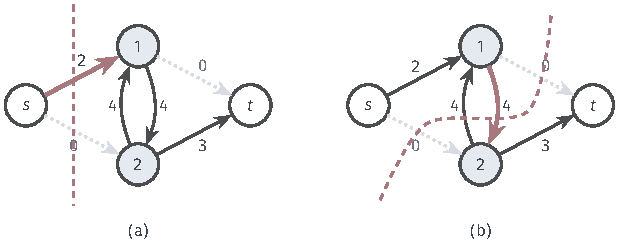
\includegraphics[width=104.687mm]{figures/01-basic-mathematics/04-graphs/tikz/c4-st-cut-construction/figure.pdf}
  \caption{两变量例子的$s$--$t$网络。弧旁数字是容量，灰色点线是容量为零的弧；红色虚线分开源侧与汇侧，红色粗弧是跨出割的正容量弧。源侧元素取$0$、汇侧元素取$1$。(a) 最小割，源侧$\{s\}$，只割断$s\to1$，容量$2$，对应$(1,1)$；(b) 源侧$\{s,1\}$，割断$1\to2$，容量$4$，对应逐点选择得到的$(0,1)$。两种情况的割容量都等于$J(\bm x)+1$。}
  \label{fig:graph-setfn-st-cut-construction}
\end{figure}

\section{算法分析}
\label{sec:graph-setfn-cut-analysis}

\paragraph{正确性}
正确性由两部分合成。由定理~\ref{thm:graph-setfn-cut-representation}，每个配置的$J$值等于对应割的容量加$K$。由第~\ref{chap:max-flow-min-cut}章的最大流最小割定理（定理~\ref{thm:graph-opt-max-flow-min-cut}）及增广路径判据（定理~\ref{thm:graph-opt-augmenting-path}），在非负容量的网络上，算法停止时残量网络中从$s$可达的集合给出一个容量等于最大流值$\Phi$的割，而任何割的容量都不小于$\Phi$。两者合起来，$\hat{\bm x}$对应的割容量最小，所以$\hat{\bm x}$是$J$的全局最小点，最小值为$\Phi+K$。

\paragraph{结果检验}
结果可以独立核对，不必相信算法实现本身。需要逐项检查四件事：
\begin{itemize}
  \item 原始成本：按原成本表直接计算$J(\hat{\bm x})$；
  \item 常数移位：重新累加各边的$\phi_{i,j}(0,0)$与各点的$m_i$，核对$K$；并逐点核对$\tilde\psi_i(0),\tilde\psi_i(1)\geq0$、各边$w_{i,j}\geq0$；
  \item 流的可行性：每条弧上$0\leq$流量$\leq$容量，每个元素顶点流入等于流出，并算出流值$\Phi$；
  \item 割容量：按跨出$S^\ast$的弧重新求和，核对它等于$\Phi$。
\end{itemize}
四项都通过时，由流值不超过割容量（引理~\ref{lem:graph-opt-weak-duality}），可行流的流值$\Phi$是一切割容量的下界，从而$\Phi+K$是一切配置成本的下界；而$J(\hat{\bm x})=\Phi+K$说明$\hat{\bm x}$达到了这个下界。流与割在这里共同充当最优性证书。

\paragraph{复杂度}
网络有$n+2$个顶点，弧数$a\leq2n+2m$，其中$m=|E|$；分解、合并一元项、移位和建弧都只需扫描一遍元素与边，用时$O(n+m)$，存储也是$O(n+m)$。

主要开销在最大流：按第~\ref{chap:max-flow-min-cut}章的分析，Edmonds--Karp算法需要$O(na^2)$次算术与比较操作，代入$a=O(n+m)$即$O(n(n+m)^2)$；换用第~\ref{sec:graph-opt-dinic}节的Dinic算法，界为$O(n^2a)=O(n^2(n+m))$。最后读出可达集合只需一次遍历，按原成本表复核$J(\hat{\bm x})$用时$O(n+m)$。

与枚举$2^n$种配置相比，这是多项式规模的计算。这里的界按顶点数与弧数计，把每次加减比较算作一步，与容量的数值无关。

\paragraph{适用范围}
若某个成对项违反式~\eqref{eq:graph-setfn-pairwise-submodular}，引理给出的$w_{i,j}$为负：这个成对项不是在惩罚取值不同，而是在奖励取值不同，而弧只能收费，不能付奖励，网络中就会出现负容量的弧。第~\ref{chap:max-flow-min-cut}章的流值与割容量的关系建立在非负容量之上，负容量时不能直接使用。

例如，奖励两个变量取值不同的成对项
\[
 \phi_{i,j}(0,1)=\phi_{i,j}(1,0)=0,\qquad \phi_{i,j}(0,0)=\phi_{i,j}(1,1)=1
\]
就违反条件：$1+1>0+0$，算出$w_{i,j}=-1$。这时的最小化一般不能化为一次最小割。所以算法~\ref{alg:graph-setfn-graph-cut}把条件写进了输入要求，构造阶段逐边检查它，不成立就报告失败，不会建出带负容量的网络。

一元项的符号则不构成限制：无论$\psi_i$取什么有限值，减去较小者后总是非负，移出的数进入常数$K$。所以容量非负只需要两件事同时成立：成对项满足次模条件，以及移位在全部边的线性部分并入之后进行。

即使每个成对项都满足条件，附加约束也会破坏这一表示。割可以任意选择源侧，所以全部$2^n$个配置都对应某个割；“恰好选$k$个”这样的数量限制只允许其中一部分配置，而最小割不受这种限制，可能落在不允许的配置上。同样不能直接套用的还有：含三个及以上变量的高阶项，以及每个变量有三种以上取值的问题。它们需要另行建模与求解；一般次模函数的最小化另有专门的算法，超出本书范围。

\paragraph{与上一章的比较}
本章与上一章都在子集上做选择，但条件和结论不同。上一章在基数或预算约束下最大化单调次模函数，算法逐轮维护已选集合，得到的是近似解，保证依赖单调性、次模性和约束的形式。本章最小化可以写成一元项加满足式~\eqref{eq:graph-setfn-pairwise-submodular}的成对项的函数，没有额外约束，算法一次性建出网络再求最小割，得到的是精确解，依据是割表示，并附带可以独立核对的证书。

\FloatBarrier
\section{本章小结}
\label{sec:pairwise-binary-chapter-summary}

本章回答了成对二值目标什么时候能不经枚举而精确最小化。目标由一元项与成对项组成，配置是$2^n$个零一向量；逐点按一元项选择会忽略成对项，一般得不到最小值。把配置看成$s$--$t$割的两侧（源侧取$0$、汇侧取$1$）后，割的每条弧都相当于一笔只在特定取值下收取的非负费用：$s\to i$对$x_i=1$收费，$i\to t$对$x_i=0$收费，一对反向弧对两者取值不同收费。

能否把目标写成这些费用之和，逐项看就清楚了。一元项减去较小值后总是非负，移出的数进入常数。成对项的四个值中，常数和只依赖单个变量的部分可以分别移出和并入一元项，剩下的相互作用$w_{i,j}$必须是取值不同时的非负惩罚，这正是成对项的次模条件$\phi_{i,j}(0,0)+\phi_{i,j}(1,1)\leq\phi_{i,j}(0,1)+\phi_{i,j}(1,0)$。条件成立时$J$作为集合函数是次模的，并且每个配置的成本等于常数$K$加对应割的容量。

算法因此分三步：逐边分解并合并一元项，全部边处理完后逐点移位得到非负容量，再求最大流并读出残量网络中从源点可达的一侧。最大流最小割定理保证读出的配置全局最优，最小值为流值加$K$。核对原始成本、常数移位、流的可行性和割容量，就能独立确认结果，不必相信算法实现。计算量是一次最大流，与枚举$2^n$种配置相比是多项式规模。

这一方法的边界也由割表示决定。成对项违反次模条件时会出现负容量，不能直接求最小割；附加“恰好选$k$个”等配置约束时，最小割可能落在不允许的配置上；含三个以上变量的高阶项或多值变量也不在这一表示之内。与上一章相比，本章得到的是精确解而不是近似解，代价是对目标结构提出了更强的要求。

许多问题的变量有更多取值，局部成本读取三个变量，或者禁止某些组合；但整体函数常常仍是只读取少数变量的局部项之和。第~\ref{part:graph-dynamic-programming}部分研究怎样借助记录读取关系的依赖图，把对全部配置的枚举化为沿图传递的小规模表格计算。

